\documentclass[12pt,letterpaper]{report}
\usepackage[margin=1in]{geometry}
\usepackage{titlesec}
\usepackage{amsmath}
\usepackage{amssymb}
\usepackage[colorlinks=true,urlcolor=black,linkcolor=black]{hyperref}
\usepackage{graphicx}
\usepackage{textcomp}
% extra packages you need
\usepackage{graphicx}
\usepackage{listings}
\usepackage{algorithm}
\usepackage{algorithmic}
\usepackage{amsmath}
\usepackage{latexsym}
\usepackage{amsfonts}
\usepackage[normalem]{ulem}
\usepackage{array}
\usepackage{amssymb}
\usepackage{subfig}
\usepackage{wrapfig}
\usepackage{wasysym}
\usepackage{enumitem}
\setlist[itemize]{after=\vspace{-0.50\baselineskip},before=\vspace{-0.95\baselineskip}}
\newlist{ucmenum}{enumerate}{1}
\setlist[ucmenum]{label=\arabic*,after=\vspace{-0.50\baselineskip},before=\vspace{-0.95\baselineskip}}
\usepackage{adjustbox}
\usepackage{ragged2e}
\usepackage{hhline}
\usepackage[svgnames,table]{xcolor}
\usepackage{tikz}
\usepackage{longtable}
\usepackage{changepage}
\usepackage{setspace}
\usepackage{multicol}
\usepackage{tabto}
\usepackage{float}
\usepackage{multirow}
\usepackage{makecell}
\usepackage{fancyhdr}
\usepackage[toc,page]{appendix}
\usepackage[utf8]{inputenc}
\usepackage{flowchart}
\usepackage{apacite}
\usepackage{color}
\makeglossaries

\titleformat{\chapter}{\bf\huge}{\thechapter}{20pt}{\huge\vspace{-.5em}}

\begin{document}
\title{Software Measurement (SOEN6611)\\[.5em]
Summer 2023\\[.5em]
Descriptive Statistics\\[.5em]
Team "Amsterdam Cartel"\\[.5em]
Deliverable 2}
\author{Unnati Chaturvedi, Mengqi Liu, Lei Zhou, Hema Reddy Mupppidi}
\maketitle

\pagenumbering{roman}
\setcounter{page}{0}

\tableofcontents

\chapter*{List of Symbols and Abbreviations}\addcontentsline{toc}{chapter}{List of Symbols and Abbreviations}



% delete these example entries
\noindent\begin{tabular}{ll}
% $\mathbb{R}$ & The set of real numbers (example)\\
% $\|\cdot\|_F$ & Frobenius norm (example)\\
GQM & Goal Question Metric\\
UC & Use Case\\
SLOC & Source Line of Codes\\
SLOC(L) & Logical SLOC\\
UCP & Use Case Point\\
PF & Productivity Factor\\
UUCP & Unadjusted Use Case Points\\
TCF & Technical Complexity Factor\\
Ecf & Environmental Complexity Factor\\
UAW & Unadjusted Actor Weight\\
UUCW & Unadjusted Use Case Weight\\
WTi & Technical Complexity Factor Weight\\
Fi & Perceived Impact Weight\\
WEi & Environmental Complexity Factor Weight


\end{tabular}

% delete this section if no figures
\listoffigures\addcontentsline{toc}{chapter}{List of Figures}
% This will automatically be populated if you included figures in your report.


% delete this section if no tables
\listoftables\addcontentsline{toc}{chapter}{List of Tables}
% This will automatically be populated if you included tables in your report.


%%%%%%%%%%%%%%%%%%%%%%%%%%%%%
\chapter{Background Information}

To develop the Sales Analytics System, named METRICSTICS, a critical system will be implemented in order to comprehensively analyze sales performance.This system will examine statistical analysis of sales data to empower the sales management team in effectively monitoring sales trends over time, conducting thorough analyses of sales history, and making informed decisions based on the insights gained. Both sales staff and sales administration personnel will have access to METRICSTICS, allowing the sales team to diligently input sales data and the sales manager to effortlessly access statistical information for specific time periods. Additionally, METRICSTICS will enable the generation of comprehensive reports on a monthly, quarterly, and yearly basis, which will be presented to the board of members.		 	 	 	

*Note: The key stakeholders for METRICSTICS are sales representatives, sales managers

%%%%%%%%%%%%%%%%%%%%%%%%%%%%%%
\chapter{Problem 3 : Use Case Points(UCP)}
\section{Effort Estimate using Use Case Point approach}
Effort Estimation using use case points is given by,
\begin{align} \label{Effort Estimate}
    Effort Estimate = UCP * PF
\end{align}

where UCP is Use Case Points, PF is Productivity Factor.

\begin{align} \label{Use Case Points}
    UCP=UUCP*TCF*ECF
\end{align}

where UUCP is Unadjusted Use Case Points, TCF is Technical Complexity Factor, ECF is Environmental Complexity Factor.

\begin{align} \label{Use Case Points}
    UUCP=UAW+UUCW
\end{align}

where UAW is Unadjusted Actor Weight, UUCW is Unadjusted Use Case Weight.

In our use case model, we have only one actor i.e; user who interacts with the system using graphical user interface. so, the actor is a complex actor with 3 points.
\begin{center}
    UAW=3
\end{center}

We have 5 classes in the system.so, it comes under average use case.
\begin{center}
    UUCW=10
\end{center}

From 2.3;
\begin{center}
    UUCP=UAW+UUCW\\
        =3+10\\
        =13\\
\end{center}


TCF concerns for the technical concerns that can impact the software project from its inspection to its conclusion, including delivery.
There are 13 different Technical Complexity Factors, each with its 
own weight.

\begin{table}[h]
    \begin{center}
    \begin{tabular}{|c|c|c|}
    \hline
          TCF Type & Description & Weight \\
    \hline\hline
    T1 & Distributed System & 2  \\
    T2 & Performance & 1 \\
    T3 & End User Efficiency & 1 \\
    T4 & Complex Internal Processing  & 1 \\
    T5 & Reusability & 1\\
    T6 & Easy to Install & 0.5 \\
    T7 & Easy to Use & 0.5\\
    T8 & Portability & 2\\
    T9 & Easy to Change & 1\\
    T10 & Concurrency & 1\\
    T11 & Special Security Features & 1\\
    T12 & Provides Direct Access for Third Parties & 1\\
    T13 & Special User Training Facilities are Required & 1\\
    \hline
    \end{tabular}
    \end{center}
    \caption{ The Technical Complexity Factors in the UCP approach.\label{example_table}}
 \end{table}

T1,T10,T11,T12,T13 has no influence;\\
T2,T3,T4 has average influence;\\
T5,T6,T7,T8,T9 has strong influence.\\

Value of no influence=0\\
Value of average influence=3\\
Value of strong influence=5\\
\begin{align} \label{Technical Complexity Factor}
    TCF=C1+(C2*\sum_{i=1}^{13} (WTi*Fi))
\end{align}
c1=0.6 and c2=0.01\\
WTi is Technical Complexity Factor Weight\\
Fi is Perceived Impact Factor.\\

From 2.4;
\begin{center}
    TCF=0.6+(0.01*((2*0)+(1*3)+(1*3)+(1*3)+(1*5)+(0.5*5)+(0.5*5)+(2*5)+(1*5)+(1*0)+\\(1*0)+(1*0)+(1*0)))\\
        =0.6+(0.01*44)\\
        =1.04
\end{center}

The purpose of ECF is to account for the development team’s personal traits, including experience. In general, the more the development team’s experience, the more the impact of ECF on UCP.

\begin{table}[h]
    \begin{center}
    \begin{tabular}{|c|c|c|}
    \hline
          TCF Type & Description & Weight \\
    \hline\hline
    E1 & Familiarity with Use Case Domain & 1.5  \\
    E2 & Part-Time Workers & -1 \\
    E3 & Analyst Capability & 0.5 \\
    E4 & Application Experience   & 0.5 \\
    E5 & Object-Oriented Experience & 1\\
    E6 & Motivation & 1 \\
    E7 & Difficult Programming Language & -1\\
    E8 & Stable Requirements & 2\\
    \hline
    \end{tabular}
    \end{center}
    \caption{The Environmental Complexity Factors in the UCP approach.\label{example_table}}
 \end{table}
Case: E1, E3, E4, E5, E6, and E8\\
0-No influence\\
1-Strong,Negative influence\\
3-Average influence\\
5-Strong,Positive influence\\

Case: E2, E7\\
0-No influence\\
1-Strong Favourable influence\\
3-Average influence\\
5-Strong, Unfavourable influence.\\

\begin{align} \label{Environment Complexity Factor}
    TCF=C1+(C2*\sum_{i=1}^{8} (WEi*Fi))
\end{align}

c1=01.4 and c2=-0.03\\
WEi is Environmental Complexity Factor Weight\\
Fi is Perceived Impact Factor.\\

From 2.5;
\begin{center}
    TCF=1.4+(-0.03*((1.5*3)+(-1*0)+(0.5*5)+(0.5*5)+(1*5)+(1*5)+(-1*1)+(2*5)))\\
        =1.4+(-0.03*28.5)\\
        =0.145
\end{center}

From 2.2;
\begin{center}
    UCP=UUCP*TCF*ECF\\
        =13*1.04*0.145\\
        =1.9604
\end{center}

From 2.1;
\begin{center}
    Effort Estimate=UCP*PF\\
        =1.9604*20\\
        =39.208
\end{center}


\section{Effort Estimate difference between using UCP approach and Actual Effort}
The difference between the estimates obtained using the Use Case Points (UCP) approach and the actual effort towards the project can vary for several reasons:\\

\textbf{Complexity Assessment}: The UCP approach relies on the subjective assessment of various factors such as actor complexity, use case complexity, technical complexity, environmental complexity, and experience factor. Depending on the accuracy of these assessments, the UCP estimate may differ from the actual effort.\\

\textbf{Changing Requirements}: During the software development lifecycle, requirements may change or evolve, leading to modifications in use cases, actors, or system complexities. If these changes are not adequately reflected in the UCP estimate, it can lead to discrepancies with the actual effort.\\

\textbf{Human Factors}: The UCP approach depends on human judgment and expertise for assessing complexity factors. Individual biases, experience levels, and interpretations can impact the accuracy of the estimation.\\

\textbf{External Factors}: Factors outside the development team's control, such as external dependencies, integration challenges, unexpected issues, or resource constraints, can affect the actual effort required, even if the UCP estimate was reasonably accurate.\\

\textbf{Skill and Efficiency}: The actual effort can be influenced by the skill and efficiency of the development team. A highly skilled and experienced team may complete the project with less effort than estimated, while a less experienced team might take longer than expected.\\

\textbf{Development Methodology}: The UCP approach assumes a traditional waterfall-style development methodology, which may not be suitable for all projects. Agile or iterative development approaches, which emphasize adaptive planning and incremental development, can have different effort dynamics.\\

\textbf{Project Management}: The effectiveness of project management practices in monitoring and controlling the development process can significantly impact the actual effort. Properly managed projects are more likely to stay on track with the estimates.\\
%%%%%%%%%%%%%%%%%%%%%%%%%%%%%%
\chapter{Problem 4 : Introduction of Project METRICSTICS}

\section{Tech Stack}
JavaFX is a powerful and versatile graphical user interface (GUI) toolkit and framework provided by Oracle for creating visually appealing and interactive desktop applications in Java. It emerged as a replacement for Swing, another GUI library for Java, and offers improved features and modern design elements to build rich and engaging user interfaces.\\

JavaFX can be used independently or alongside other Java technologies, such as Java Swing and Java 2D, to extend the functionality of Java applications. It provides a modern and versatile approach to building desktop applications, making it a popular choice for Java developers seeking to create dynamic and visually appealing user interfaces.\\

Key features of JavaFX include:\\

\textbf{Rich UI Controls:} JavaFX provides a wide range of pre-built UI controls such as buttons, text fields, labels, tables, charts, and more, making it easier to create feature-rich and intuitive interfaces. \\

\textbf{Scene Graph:} JavaFX utilizes a scene graph to represent the hierarchical structure of elements in the user interface. This approach allows for efficient rendering and manipulation of visual components. \\

\textbf{CSS Styling:} Styling in JavaFX is done using Cascading Style Sheets (CSS), just like web development. This separation of style from the application logic promotes better code organization and maintainability. \\

\textbf{FXML:} JavaFX supports FXML, an XML-based markup language that allows developers to define the user interface layout separately from the application logic. This enables a clear separation of concerns, making it easier for designers and developers to collaborate. \\

JavaFX includes powerful animation support, allowing developers to create smooth and visually appealing transitions and effects for their applications. \\


\begin{figure}
    \begin{center}
    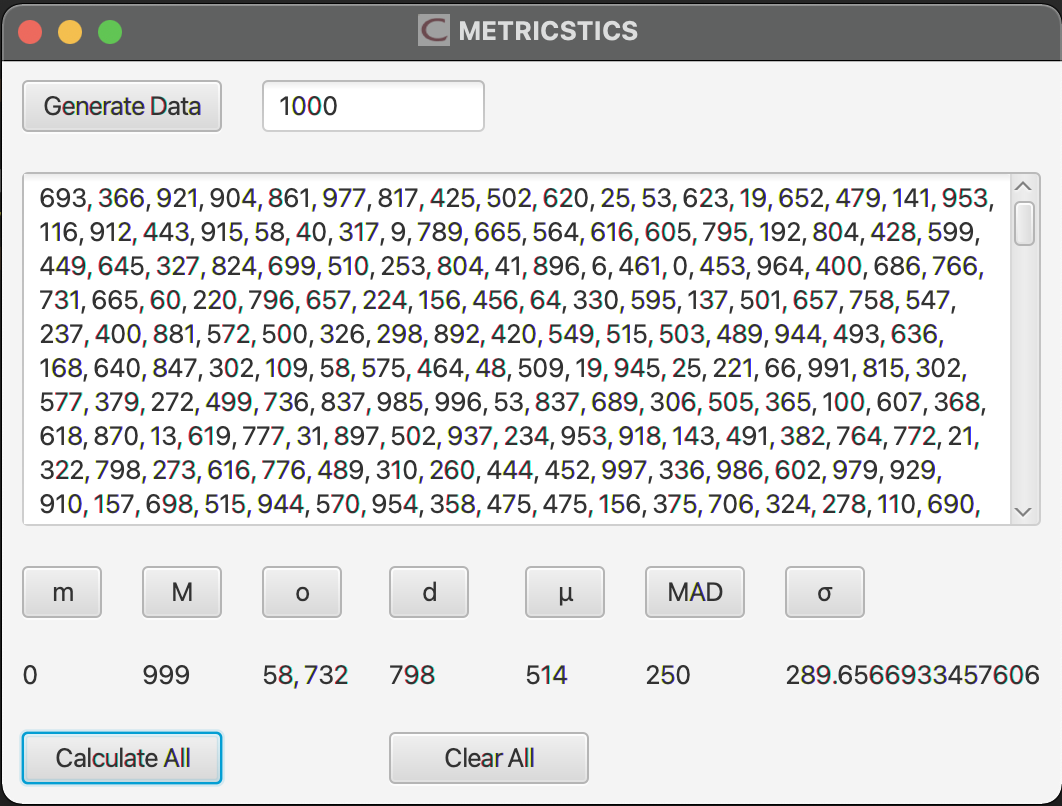
\includegraphics[width=0.5\linewidth]{app.png}
    \end{center}
       \caption{METRICSTICS Application \label{METRICSTICS Application}}
\end{figure}

\begin{figure}
    \begin{center}
    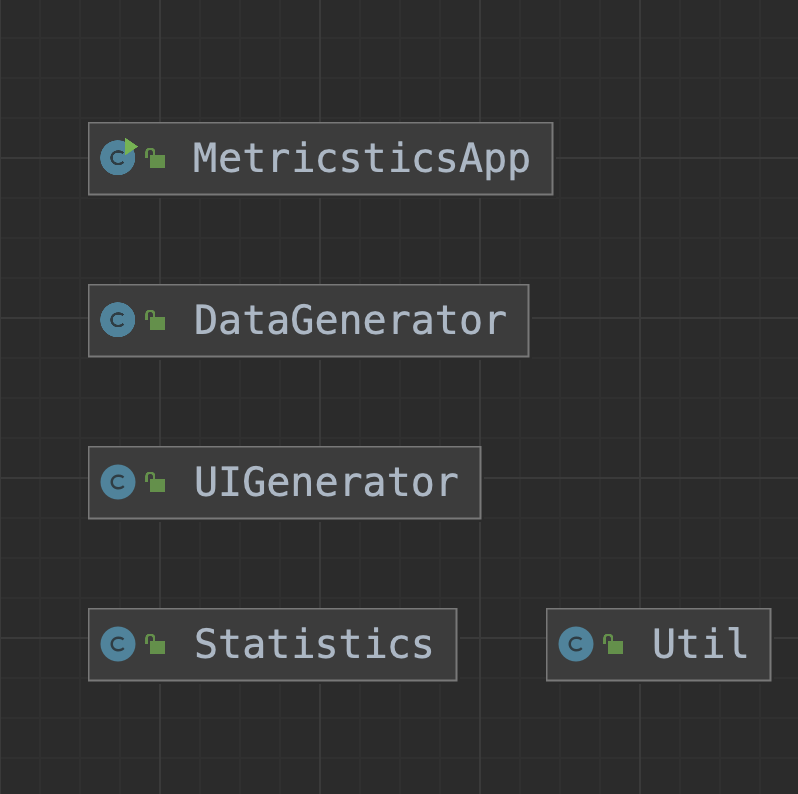
\includegraphics[width=0.5\linewidth]{classes.png}
    \end{center}
       \caption{Java Classes \label{Java Classes}}
\end{figure}

\begin{figure}
    \begin{center}
    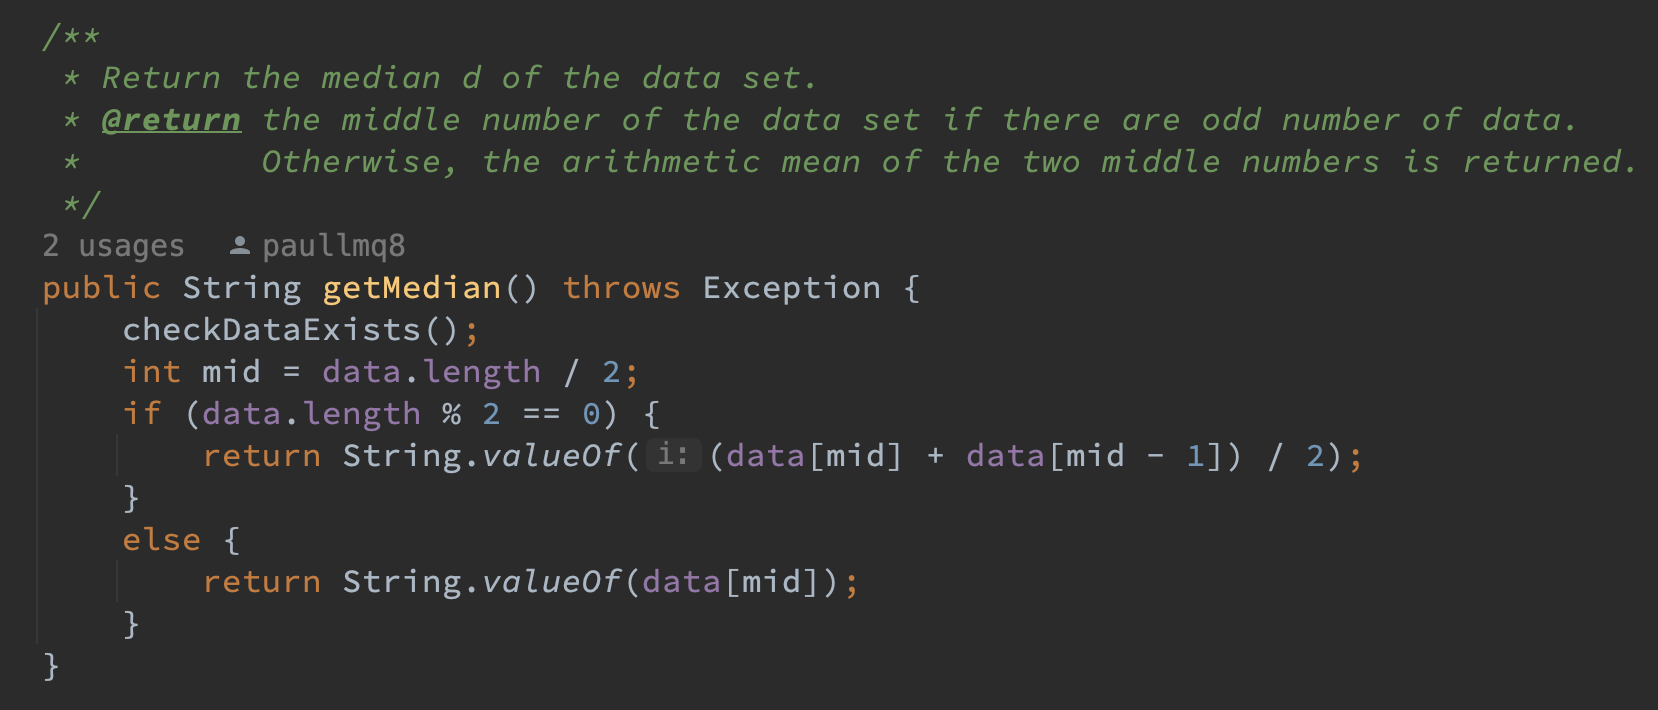
\includegraphics[width=0.5\linewidth]{code_sample.png}
    \end{center}
       \caption{Code Sample \label{Code Sample}}
\end{figure}


%%%%%%%%%%%%%%%%%%%%%%%%%%%%%%
\chapter{Problem 5 : Cyclomatic number}
\section{Cyclomatic number}
 In this application, three distinct classes, namely MetricsticsApp, Statistics, and DataGenerator, have been implemented, with each assuming responsibility for distinct and specific functionalities. The MetricsticsApp class assumes the role of drawing and defining the interface for calculators, while the Statistics class is responsible for defining statistical functions. Lastly, the DataGenerator class fulfills the crucial task of generating data for the application.\\

 To obtain the cyclomatic complexity for each class and its corresponding values, I utilized a tool known as **CodeMetrics**. This tool aids in analyzing the complexity of software code by calculating the cyclomatic number, which provides valuable insights into the code's structural intricacies and potential points of concern.\\

 Here is the Cyclomatic number for each methods: \\
 
 \begin{itemize}
 \item \textbf{MetricsticsApp}:
    \begin{itemize}
        \item main() - 1
        \item start() - 1
    \end{itemize}
 \end{itemize}

 \begin{itemize}
 \item \textbf{DataGenerator}: 
    \begin{itemize}
        \item generate() - 4
    \end{itemize}
 \end{itemize}

 \begin{itemize}
 \item \textbf{Statistics}: 
    \begin{itemize}
        \item setData() - 1
        \item clear() - 1
        \item checkDataExists() - 6
        \item getMin() - 5
        \item getMax() - 5
        \item getMode() - 11
        \item getMedian() - 10
        \item getArithmeticMean() - 4
        \item getMeanAbsoluteDeviation() - 5
        \item getStandardDeviation() - 8
        \item abs() - 4
        \item sqrt() - 26
        \item calculateAndDisplay() - 10
        \item calculateAll() - 1
    \end{itemize}
 \end{itemize}

 \begin{itemize}
 \item \textbf{UIGenerator}: 
    \begin{itemize}
        \item generator() - 11
        \item start() - 3
    \end{itemize}
 \end{itemize}

 \begin{itemize}
 \item \textbf{Util}:  
    \begin{itemize}
        \item createOpertorButton() - 2
        \item clearAll() - 1
    \end{itemize}
 \end{itemize}

[some screen short attached below]

\section{Conclusions for each classes}
\textbf{MetricsticsApp Class}: MetricsticsApp is driver class of this application, the cyclomatic complexity of both methods in the MetricsApp class is low, with each method having a value of 1. In this case, both methods have a simple control flow with a single path, making them relatively easy to comprehend and maintain.\\
 
\textbf{UIGenerator Class}: 
The DataGenerator class exhibits slightly higher complexity than the MetricsApp class, with a cyclomatic number of 11 and 3. This difference can be attributed to the generate() method, which follows a recurring UI creation pattern utilizing various variables and parameters. To enhance code quality and reduce the cyclomatic complexity, it is advisable to refactor the method using the Factory Method pattern.\\

\textbf{Statistics Class}: 
The Statistics class has a highest Cyclomatic complexity among of others, indicating the presence of numerous decision points and complex control flow. For majority of the method in Statistics class, it is below 10, which indicate multiple decision points and branching paths. Howevevr, there is one method sqrt() holds 26 cyclomatic number, which need to refactor in order to reduce complexity and organizing control flow can make the code more readable and easier to maintain.\\

\textbf{DataGenerator Class}: 
 The DataGenerator class has a moderate Cyclomatic complexity of 5, indicating a moderate level of control flow complexity. The class comprises only one method, generate(), which generates random numbers, and its Cyclomatic complexity is 4. Due to the straightforward nature of the class and method, they are likely to be easy to maintain and comprehend.\\

\textbf{Util Class}: The Util class exhibits a low Cyclomatic complexity of 2 and 1 for each of its methods. This suggests a relatively simple control flow, contributing to the class's ease of comprehension and maintainability. The class adheres to the principle of single responsibility by decomposing UI components into separate methods, further enhancing its clarity and structure. \\

\begin{figure}
    \begin{center}
    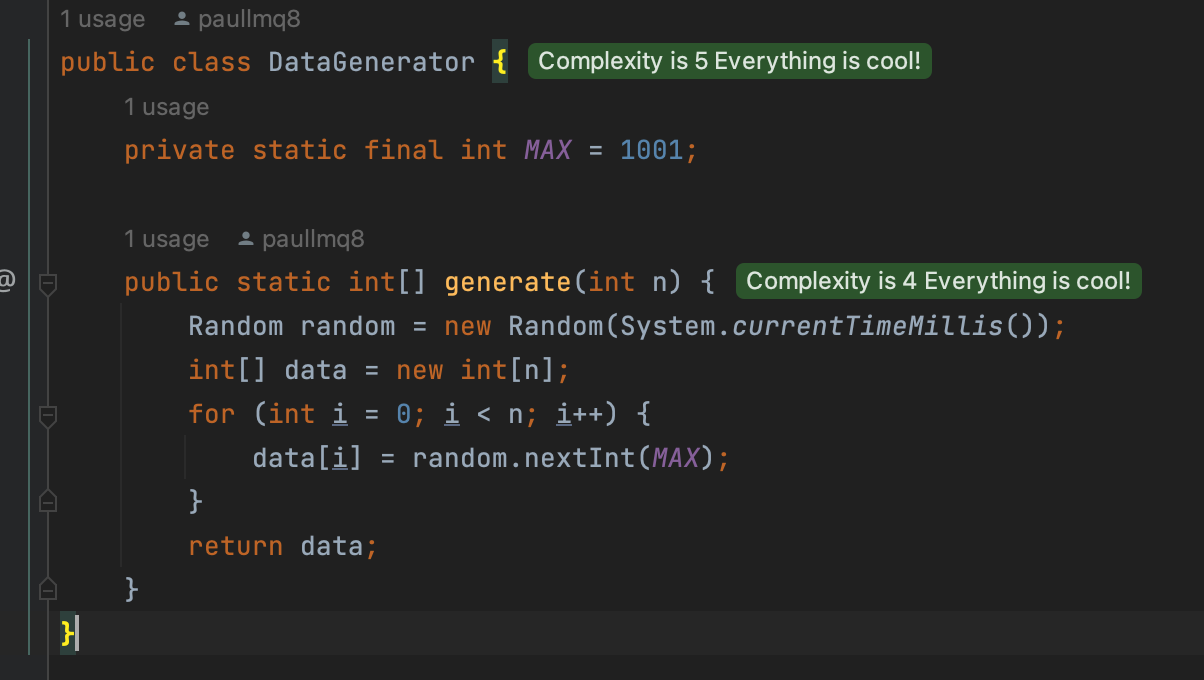
\includegraphics[width=0.5\linewidth]{cc1.png}
    \end{center}
       \caption{Cyclomatic Number Code Sample \label{Code Sample}}
\end{figure}

\begin{figure}
    \begin{center}
    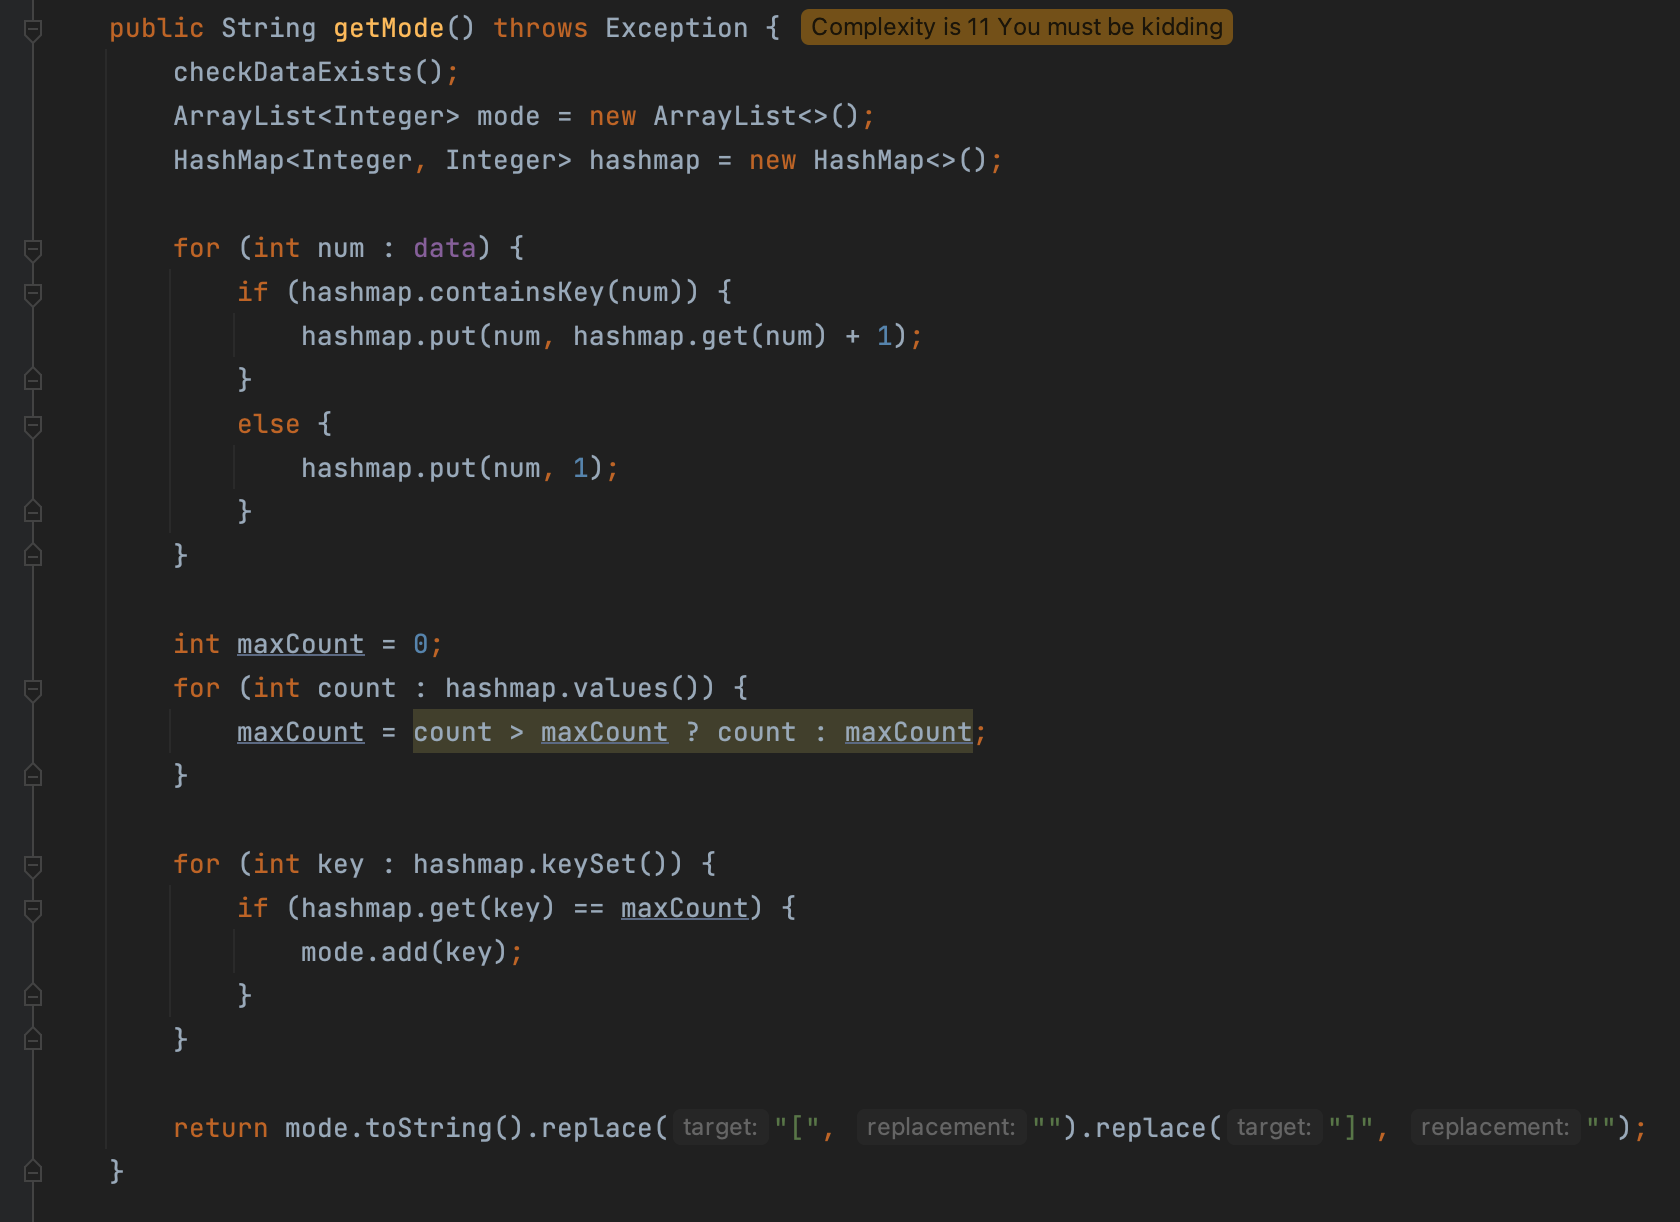
\includegraphics[width=0.5\linewidth]{cc2.png}
    \end{center}
       \caption{Cyclomatic Number Code Sample \label{Code Sample}}
\end{figure}

\begin{figure}
    \begin{center}
    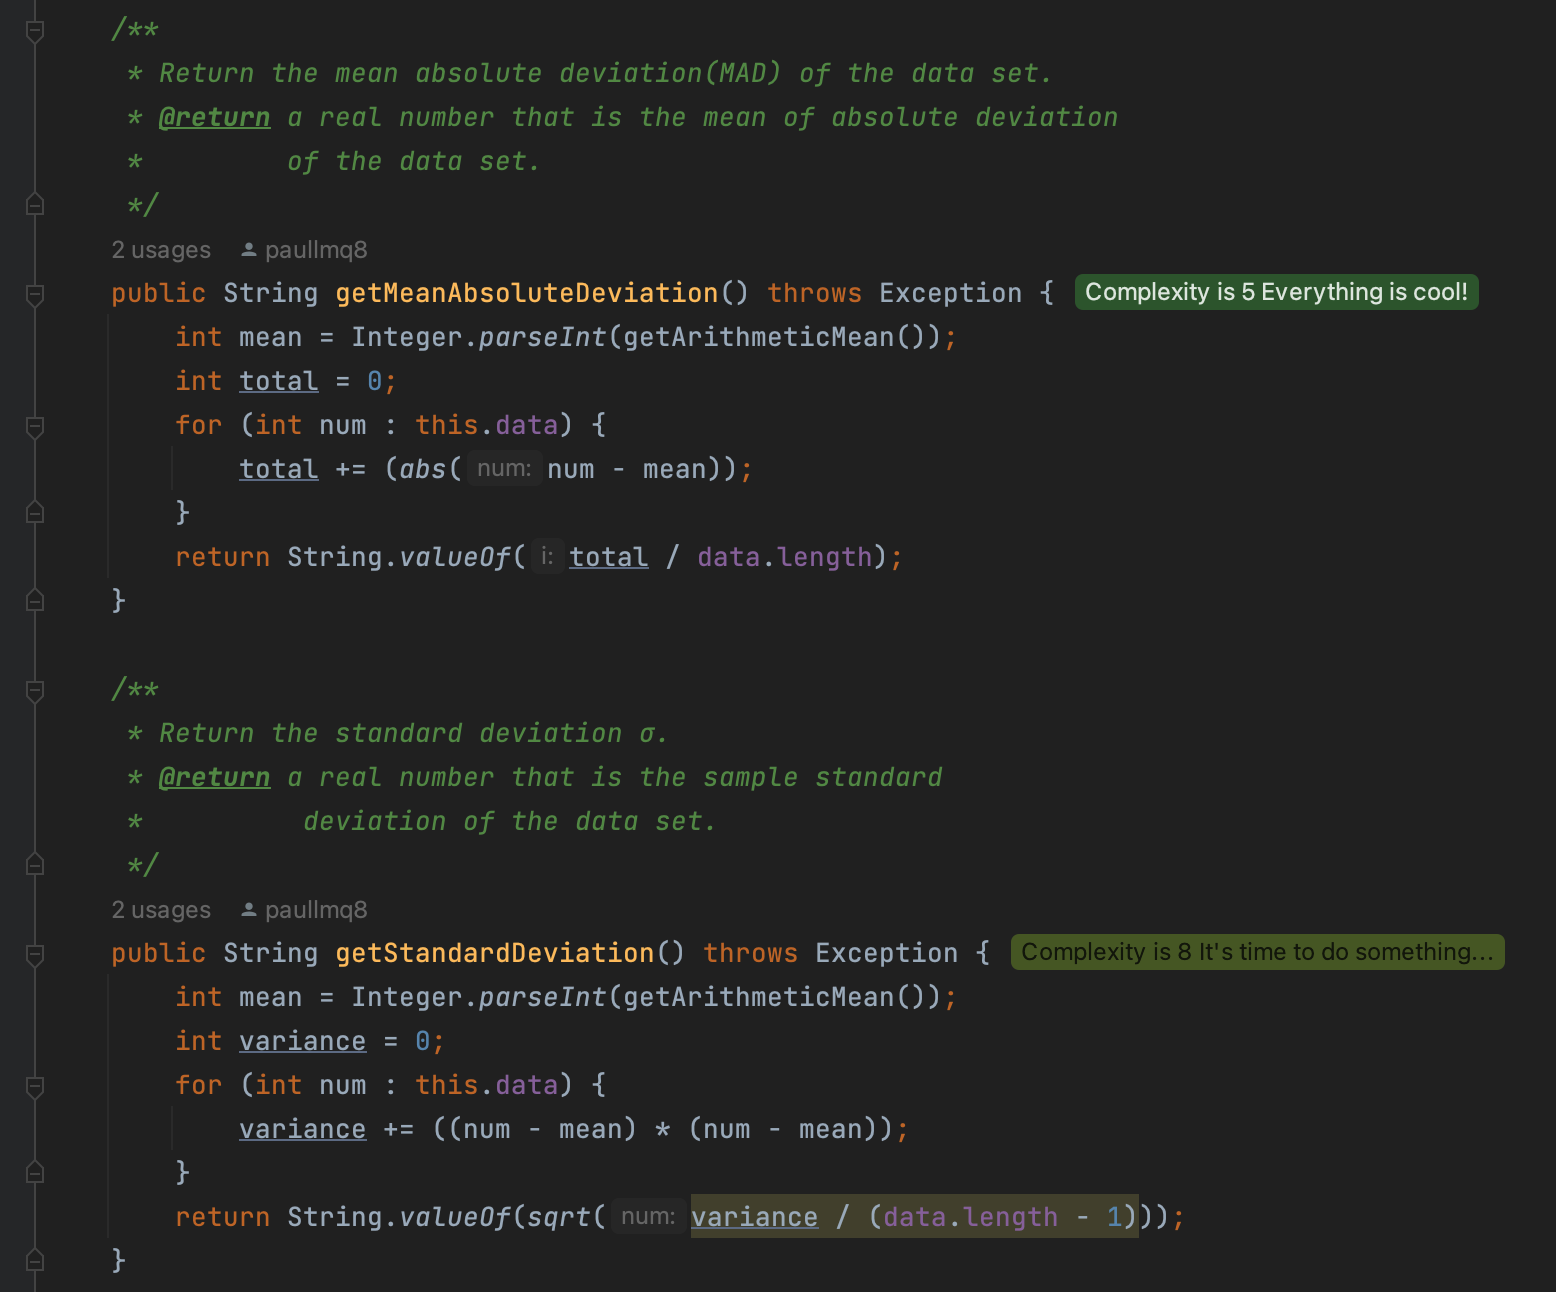
\includegraphics[width=0.5\linewidth]{cc3.png}
    \end{center}
       \caption{Cyclomatic Number Code Sample \label{Code Sample}}
\end{figure}

\begin{figure}
    \begin{center}
    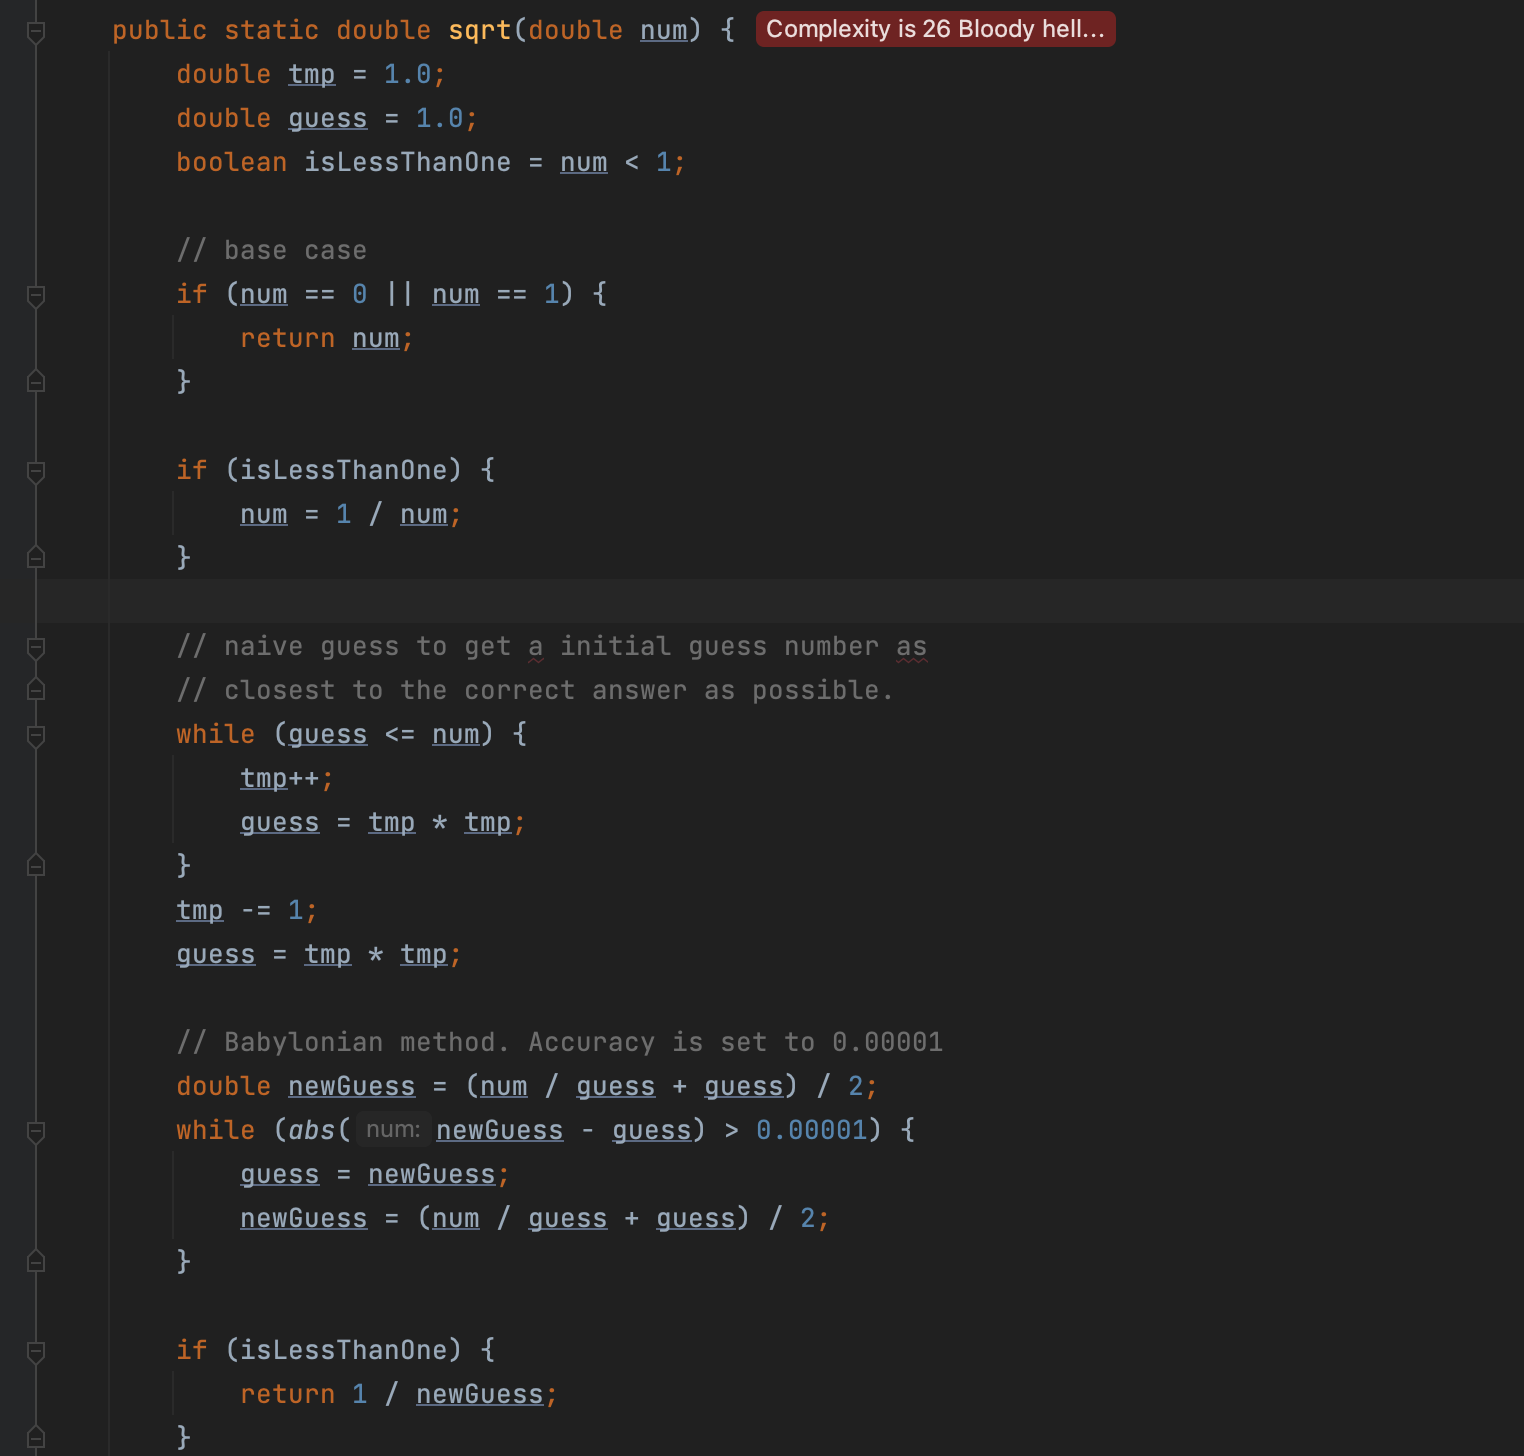
\includegraphics[width=0.5\linewidth]{cc4.png}
    \end{center}
       \caption{Cyclomatic Number Code Sample \label{Code Sample}}
\end{figure}

\begin{figure}
    \begin{center}
    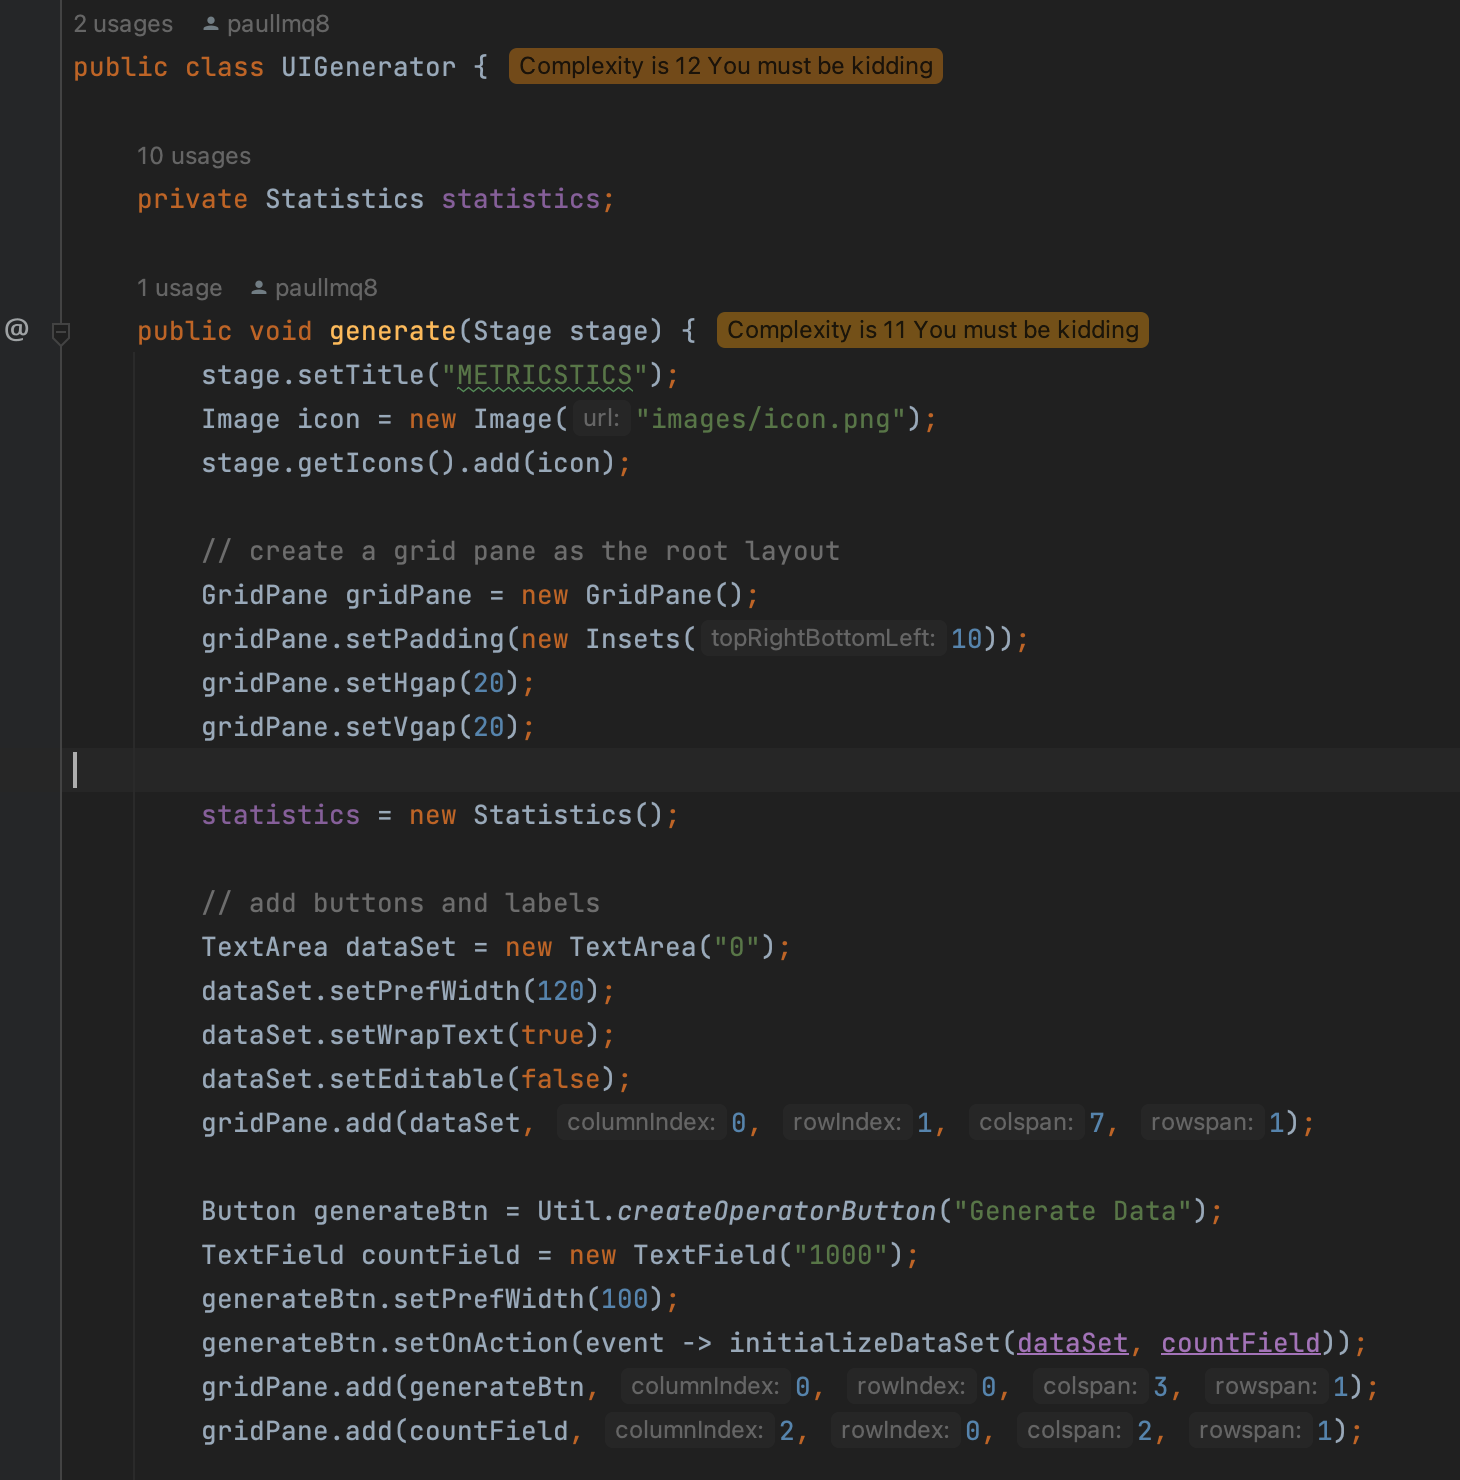
\includegraphics[width=0.5\linewidth]{cc5.png}
    \end{center}
       \caption{Cyclomatic Number Code Sample \label{Code Sample}}
\end{figure}


%%%%%%%%%%%%%%%%%%%%%%%%%%%%%%
\chapter{Problem 6 : WMC, CF, LCOM}

\section{WMC}
The formula of WMC is to obtain the sum of weighted method per class. In this senicaio(Non-Normalization case), we will use we have cyclomatic numbers above to calculate the WMC\\

\begin{itemize}
     \item WMC(MetricsticsApp)  —  1 + 1 = 2
     \item WMC(DataGenerator) — 4
    
     \item WMC(Statistics) — 6 + 5 + 5 + 11 + 10 + 4 + 5 + 8 + 4 + 26 = 84
    
     \item WMC(UIGenrator) — 11 + 3 = 14
    
     \item WMC(Util) — 2 + 1 = 3
\end{itemize}

\textbf{MetricsticsApp}: It has a relatively low WMC of 2, which suggests that the class has a simple structure with only two methods, making it easy to understand and maintain\\

\textbf{DataGenerator}: With a WMC of 4, the DataGenerator class has a moderate complexity, indicating that it contains a few methods, but they are not overly complex. It should still be relatively straightforward to manage.\\

\textbf{Statistics}: The Statistics class has a high WMC of 84, signifying significant complexity due to a large number of methods and their complexities. This class may require careful attention during development and maintenance to ensure its correctness and readability.\\

\textbf{UIGenerator}: The UIGenerator class has a moderate WMC of 14, indicating that it is not excessively complex but still requires attention to maintain and understand the class.\\

\textbf{Util}: With a WMC of 3, the Util class has relatively low complexity. It contains a few methods, making it straightforward to handle and likely follows the principle of single responsibility

In summary, the complexity levels vary among the classes. While some classes have low complexity and are easy to maintain, others exhibit higher complexity, necessitating careful review and potential refactoring to improve code quality and readability. Developers should focus on managing the complexity of high WMC classes, especially the Statistics class with its WMC of 84, to ensure that it remains maintainable and comprehensible over time.


\section{CF}
By Figure 5.1, n = 6, (0+0+1+1+1+1)/(36 - 6) = 2/15 = 0.133333333333 

the low coupling factor suggests that the software system's design encourages a well-structured and loosely connected architecture, which is beneficial for software development and maintenance,
A coupling factor of 0.133333333333 signifies that the components or modules within the software system are loosely connected, with minimal dependencies between them

\section{LOCM}

 \smallskip
 \hspace{5mm}
 \textbf{LCOM(MetricsticsApp)}: (Figure 5.2)
 \vspace{1mm}
 \text{m = 2, a = 2} 
    \begin{itemize}
        \item \(\mu\) (Stage) = 1
        \item \(\mu\) (Application) = 1
    \end{itemize} 
    \vspace{5mm} \hspace{7mm} \text{LCOM(MetricsticsApp) =  [(1/2) * (1+1) - 2)] / 1 - 2 = 1 }
    \space
    
 \bigskip
 \textbf{LCOM(UIGenerator)}: (Figure 5.3) 
 \text{m = 2, a = 9 }
    \begin{itemize}
        \item \(\mu\) (Stage) = 1
        \item \(\mu\) (Image) = 1
        \item \(\mu\) (GridPane) = 1
        \item \(\mu\) (Textarea) = 2
        \item \(\mu\) (Button) = 1
        \item \(\mu\) (Label) = 1
        \item \(\mu\) (Scene) = 1
        \item \(\mu\) (Alert) = 1
        \item \(\mu\) (Statistics) = 1
    \end{itemize} 
    \vspace{5mm} \hspace{7mm} 
    LCOM(Statistics) = [(1/9) * (1+1+1+2+1+1+1+1+1) - 2] / (1-2) = 8/9 = 0.888889
    \space

 \bigskip
 \textbf{LCOM(DataGenerator)}: (Figure 5.4) 
 \text{m = 1, a = 3 }
    \begin{itemize}
        \item \(\mu\) (Random) = 1
        \item \(\mu\) (Max) = 1
        \item \(\mu\) (System) = 1
    \end{itemize} 
    \vspace{5mm} \hspace{7mm} 
    LCOM(DataGenerator) = [(1/3) * (1+1+1) - 1] / (1 - 1) = 0    
    \space


 \bigskip
 \textbf{LCOM(Statistics)}: (Figure 5.5) 
 \text{m = 12, a = 4 }
    \begin{itemize}
        \item \(\mu\) (data) = 8
        \item \(\mu\) (number) = 2
        \item \(\mu\) (Alert) = 2
        \item \(\mu\) (Label) = 1
    \end{itemize} 
    \vspace{5mm} \hspace{7mm} 
    LCOM(Statistics) = [(1/4) * (8+2+2+1) - 12] / (1 - 12) = (35/4)/11 = 0.795454545455
    \space


 \bigskip
 \textbf{LCOM(Util)}: (Figure 5.6) 
 \text{m = 2, a = 2 }
    \begin{itemize}
        \item \(\mu\) (Button) = 1
        \item \(\mu\) (Label) = 1
    \end{itemize} 
    \vspace{5mm} \hspace{7mm} 
    LCOM(Util) = [(1/2) * (1+1) - 1] / (1 - 2) = 1
    \space

\vspace{5mm}
\textbf{Conclusion} \\

\text{There 5 different LOCM value, 1, 0.888889, 0, 0.795454545455, 1}

\begin{itemize}
        \item MetricsticsApp has an LCOM of 1, indicating good cohesion, meaning its methods are well-related and work together effectively.
        \item UI has an LCOM of 0.888889, which is close to 1, suggesting reasonable cohesion, but some methods might not be as closely related to others.
        \item DataGenerator has an LCOM of 0, meaning the methods in the class are highly cohesive, and they likely work closely together.
        \item Statistics has an LCOM of 0.795454545455, which is relatively close to 1, suggesting decent cohesion but with some room for improvement.
        \item Util has an LCOM of 1, indicating good cohesion, implying its methods are well-organized and work together effectively.
    \end{itemize} 
\vspace{10mm} In summary, most of the classes exhibit reasonable to good cohesion based on their LCOM values. However, the Statistics class might benefit from a bit more organization to improve its cohesion further. 















\begin{figure}
    \begin{center}
    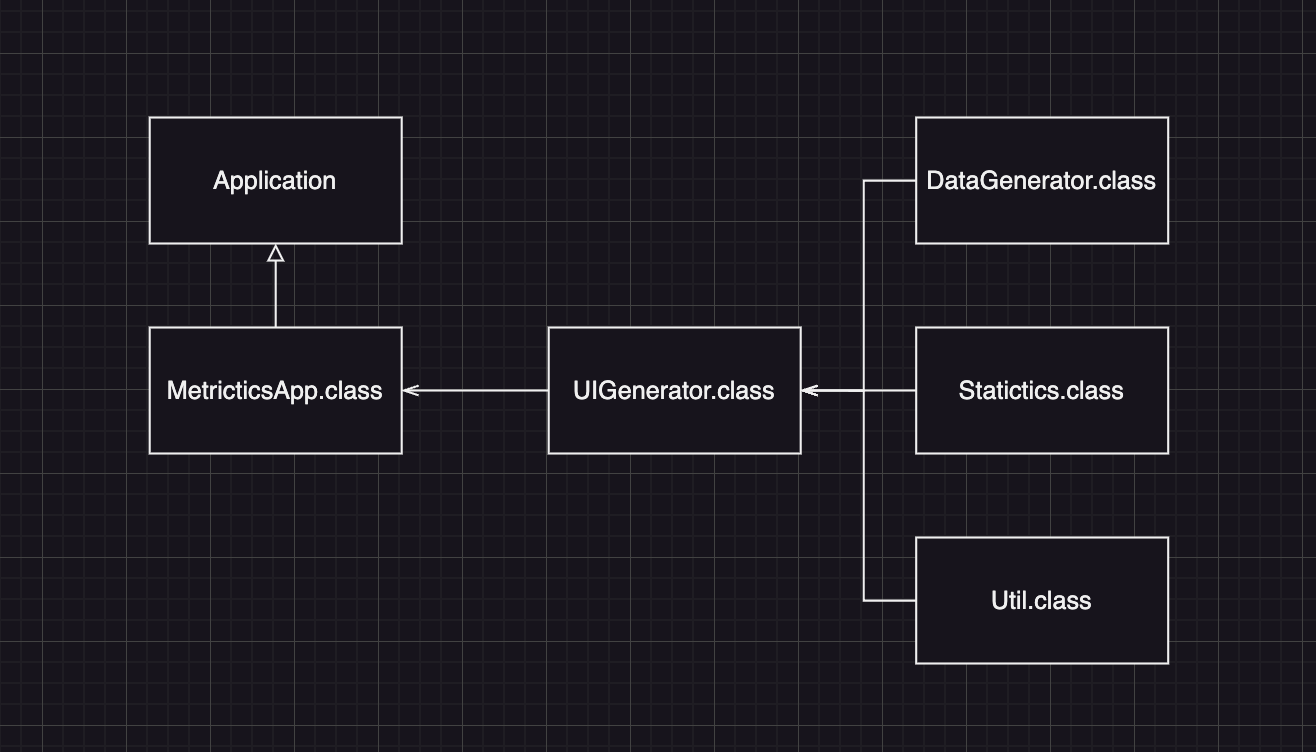
\includegraphics[width=0.5\linewidth]{CF.png}
    \end{center}
       \caption{CF \label{Code Sample}}
\end{figure}

\begin{figure}
    \begin{center}
    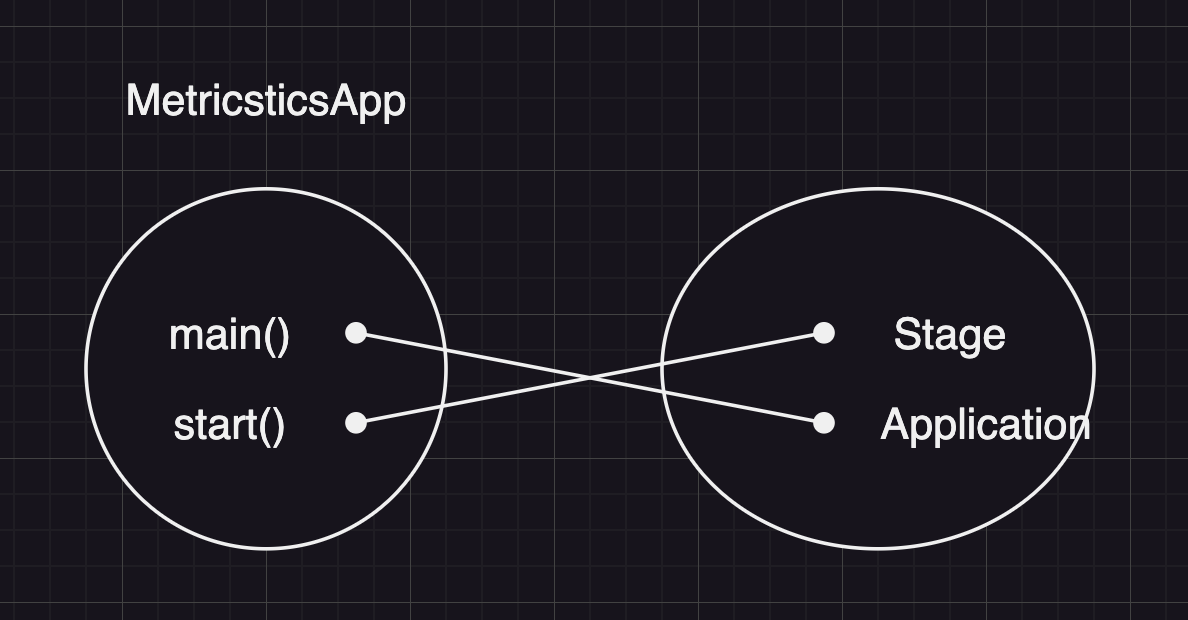
\includegraphics[width=0.5\linewidth]{LCOM1.png}
    \end{center}
       \caption{LCOM MetricsticsApp \label{Code Sample}}
\end{figure}

\begin{figure}
    \begin{center}
    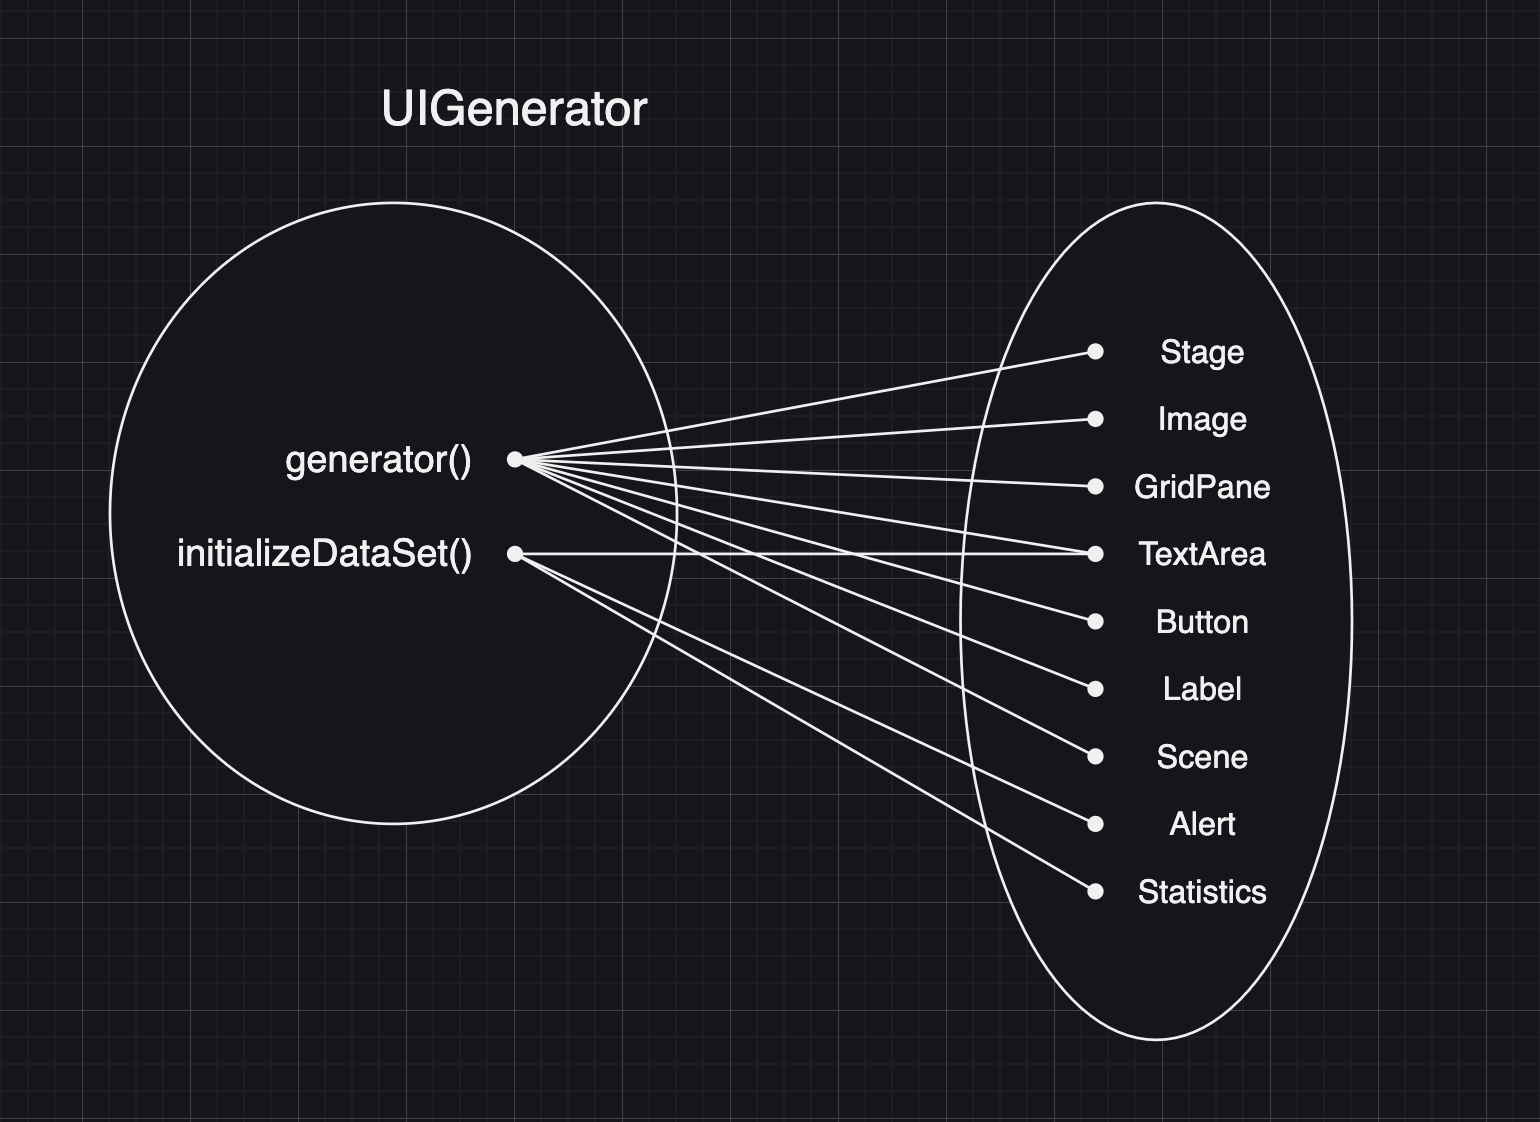
\includegraphics[width=0.5\linewidth]{LCOM2.png}
    \end{center}
       \caption{LCOM UIGenerator \label{Code Sample}}
\end{figure}

\begin{figure}
    \begin{center}
    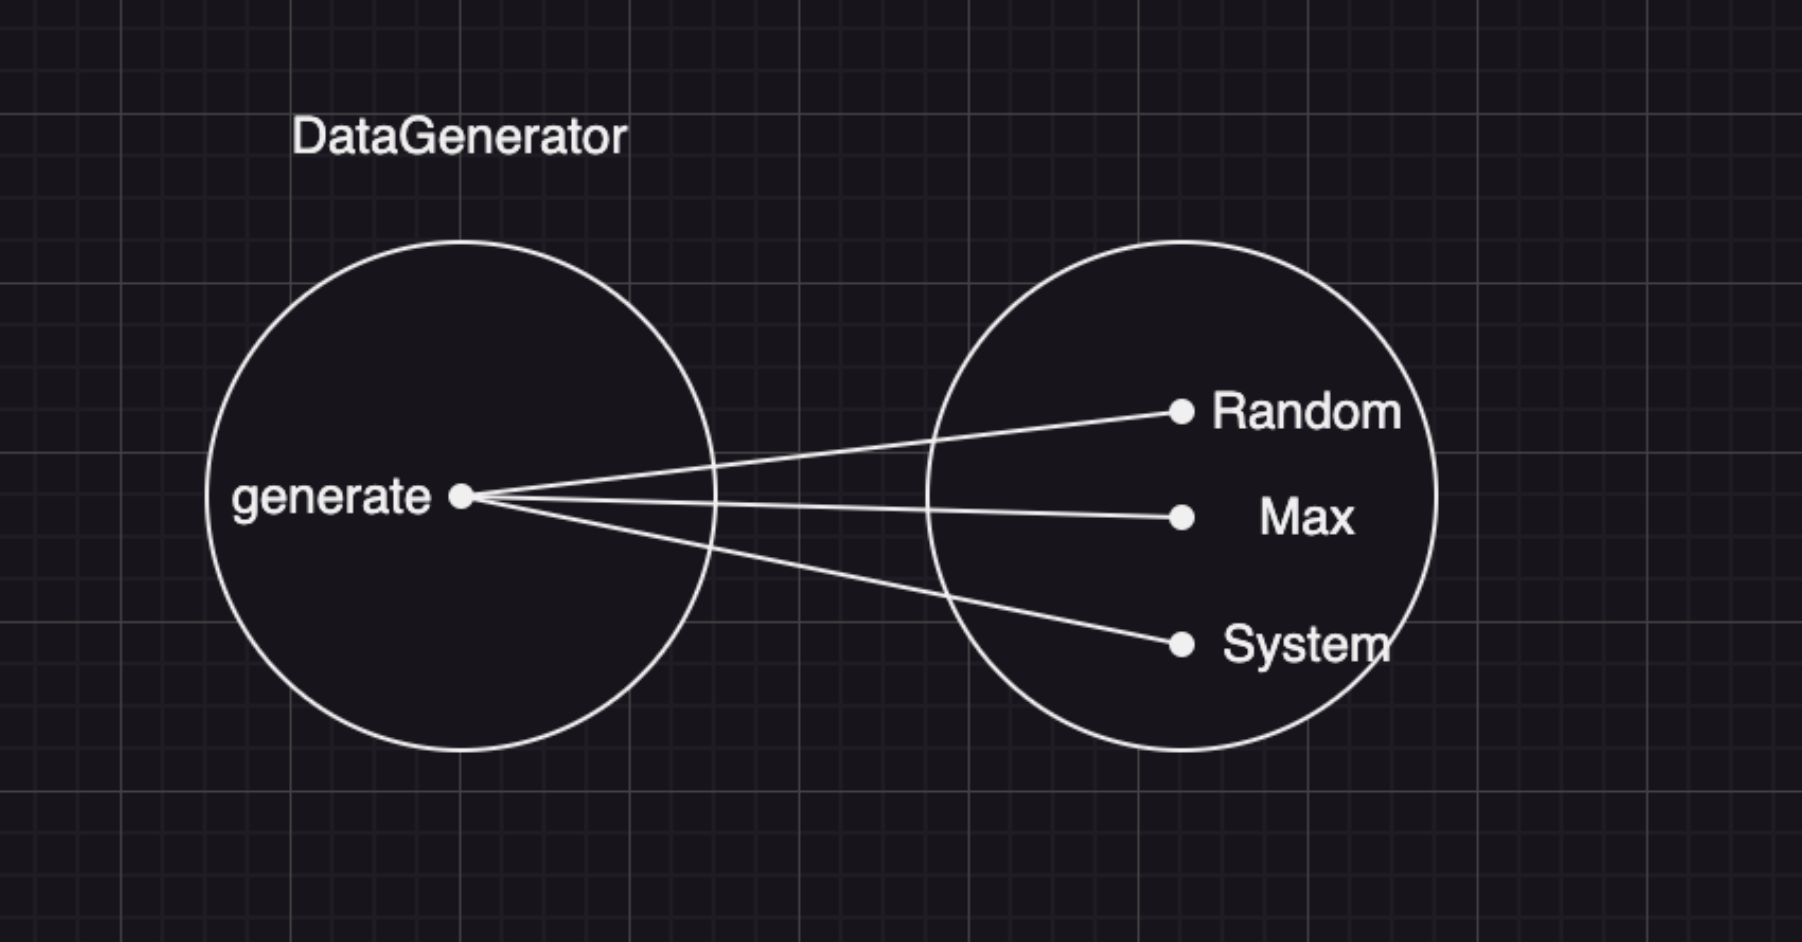
\includegraphics[width=0.5\linewidth]{LCOM3.png}
    \end{center}
       \caption{LCOM DataGenerator \label{Code Sample}}
\end{figure}

\begin{figure}
    \begin{center}
    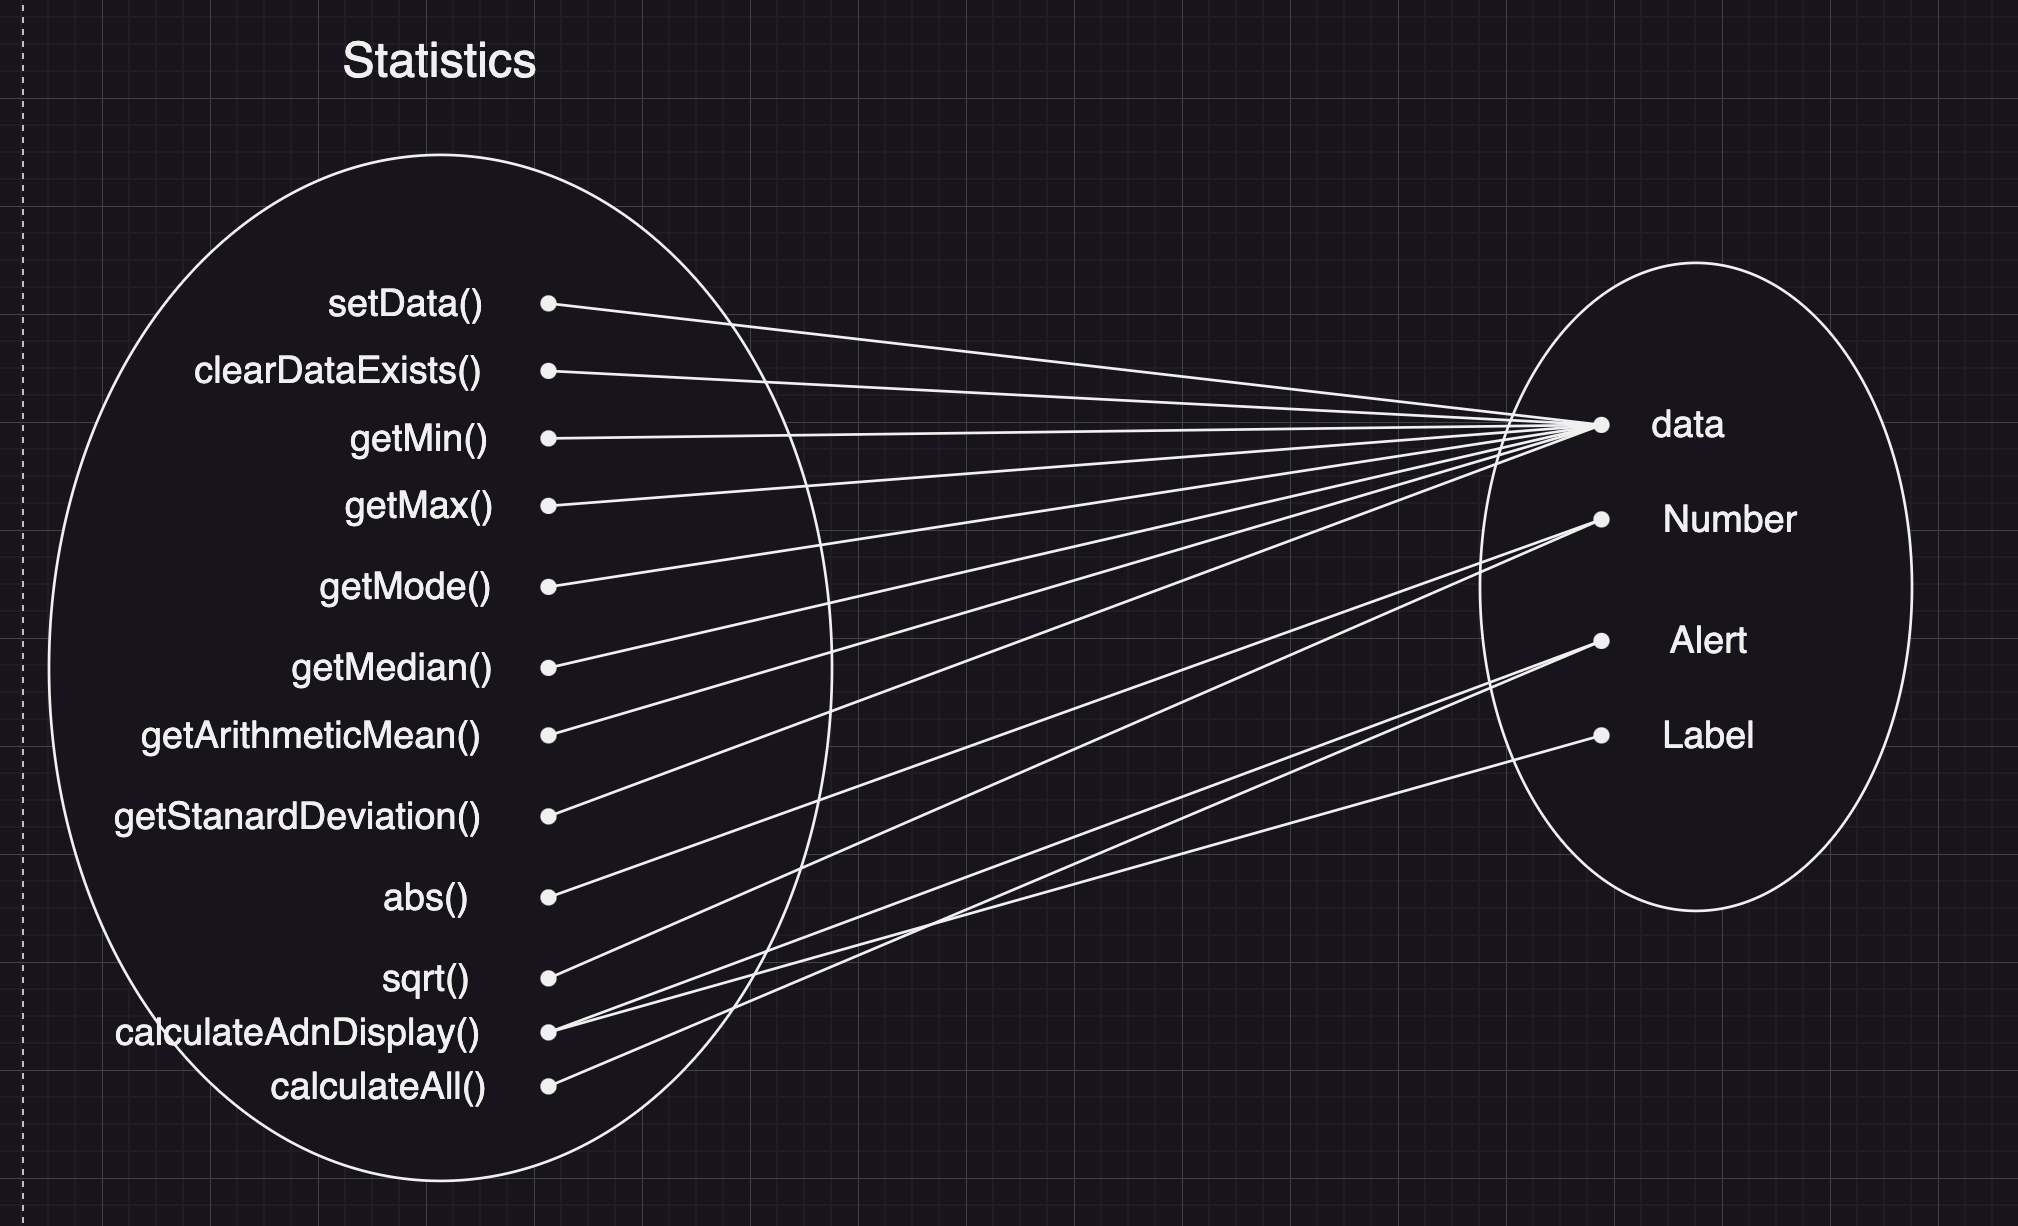
\includegraphics[width=0.5\linewidth]{LCOM4.png}
    \end{center}
       \caption{LCOM Statistics \label{Code Sample}}
\end{figure}




\begin{figure}
    \begin{center}
    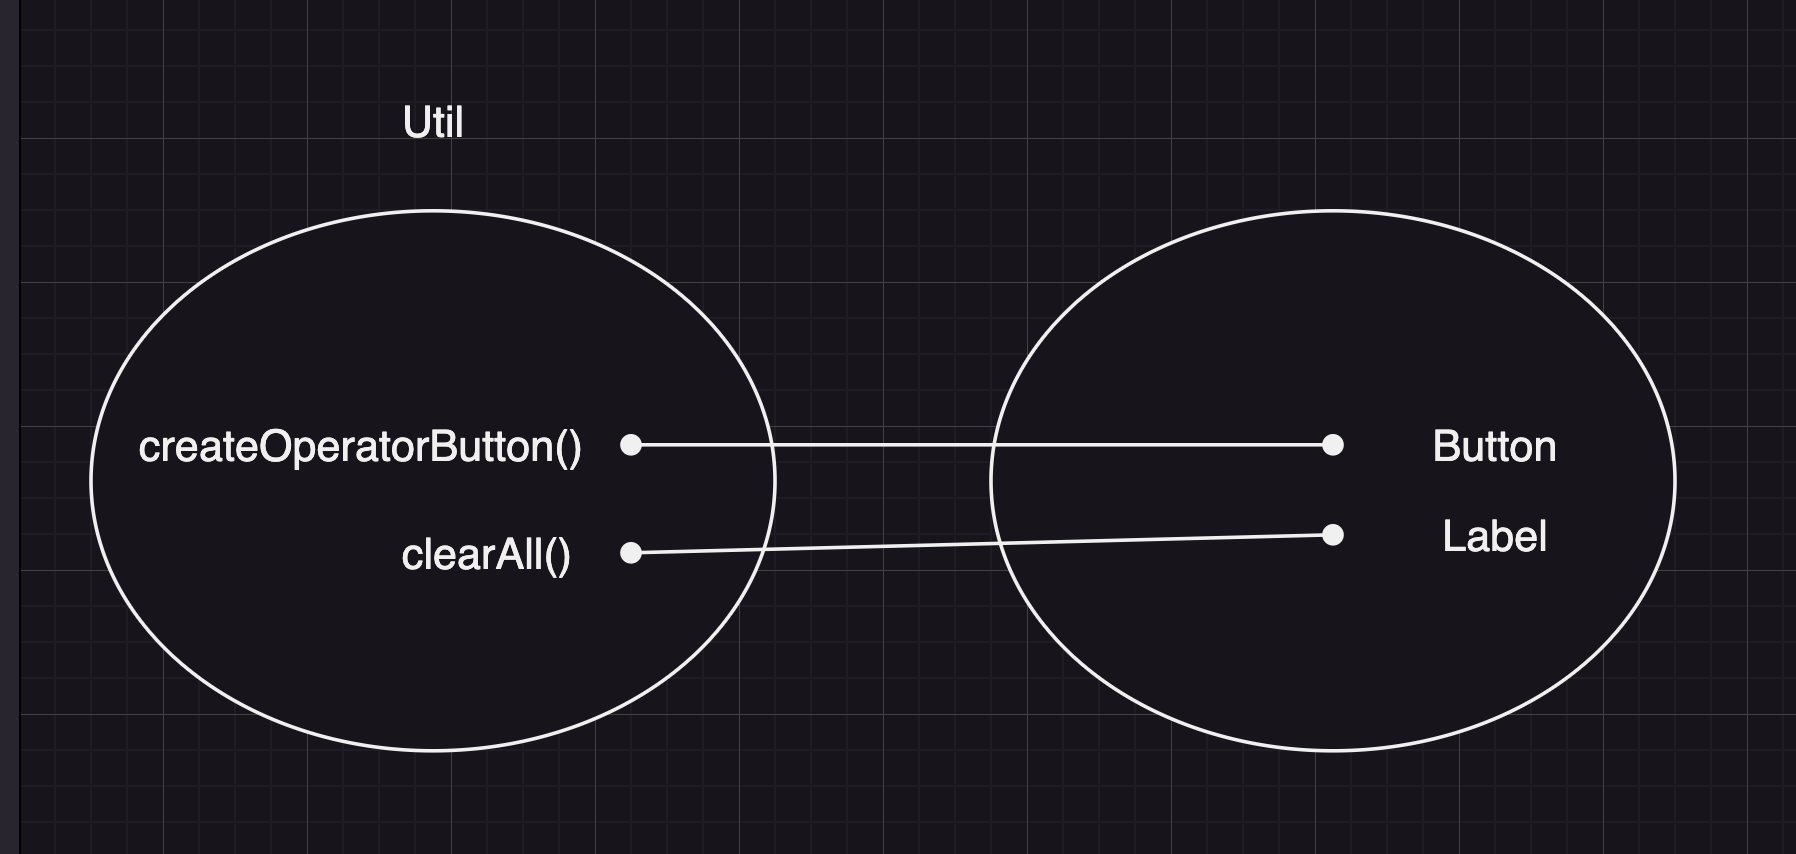
\includegraphics[width=0.5\linewidth]{LCOM5.png}
    \end{center}
       \caption{LCOM Util \label{Code Sample}}
\end{figure}



%%%%%%%%%%%%%%%%%%%%%%%%%%%%%%
\chapter{Problem 7 : Physical And Logical SLOC}

\section{Goal}

Calculating the Physical SLOC and Logical SLOC for METRICSTICS. For Physical SLOC a tool named CLOC is used and for Logical SLOC a manual counting approach was applied.\\

\section{Physical SLOC}
refers to the number of lines in the source code of a software project that contain executable statements, meaning lines that have actual code instructions and are not blank lines or comments.[Chatgpt]
\\

\textbf{Tool-CLOC}: CLOC is used to count blank lines, comment lines, and physical lines of source code in many programming languages. This project uses the CLOC tool to calculate the physical SLOC.\\

\textbf{Installing CLOC}: CLOC documentation provides numerous way to install the tool. Installing via package manager can vary depending on the operating system.
"npm install -g cloc " can be used to globally install the tool on your terminal.\\

\textbf{Using CLOC}: CLOC provides a very user friendly and simple command line tool. To calculate the physical SLOC the main directory was selected and using the command "cloc main" provides the user with a report.  \\

\begin{figure}
    \begin{center}
    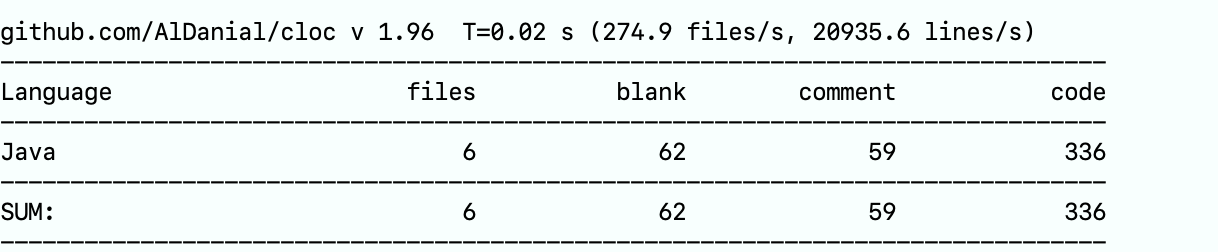
\includegraphics[width=1\linewidth]{cloc.png}
    \end{center}
       \caption{Physical SLOC \label{Physical SLOC}}
\end{figure}
\
\textbf{Advantages of Physical SLOC}: Physical SLOC is language-independent. SLOC also offer insights into code size and complexity.  \\
\\
\textbf{Inference}: 336 Lines of code indicates a smaller size system. The SLOC value of this project suggests less complexity and due to its small size it would be easier to maintain.



\section{Logical SLOC}
It is a measure of the size or complexity of a software project based on the number of logical statements or instructions in the source code that affect the program's control flow or behavior
\\

\textbf{Manual Method}: The project's logical SLOC is calculated manually. following the UCC (Unified Code Counter ) Logical SLOC Counting Rules for Java.The rules are shown in Figure 4.2 and 4.3. Total SLOC(L) is a summation of SLOC(L) of all classes present in the system. The total Logical SLOC is 83 \\
\begin{itemize}
 \item Total logical SLOC(MetricsticsApp): 9
     \\
     \begin{itemize}
     \item Package declaration: 1 SLOC
    \item Import statements: 3 SLOCs
    \item Class declaration (MetricsticsApp): 1 SLOC
    \item main method: 1 SLOC
    \item launch method call: 1 SLOC
    \item start method: 1 SLOC
    \item Instantiation of UIGenerator class: 1 SLOC
   \\
  \end{itemize}
 \end{itemize}
\begin{itemize}
      \item Total logical SLOC(DataGenerator): 6
      \\
       \begin{itemize}
    \item Import statements: 2 SLOCs
    \item Class declaration (DataGenerator): 1 SLOC
    \item Constant declaration (MAX): 1 SLOC
    \item Method declaration (generate): 1 SLOC
    \item For loop: 1 SLOC
    \\
  \end{itemize}
\end{itemize}

\begin{itemize}
     \item Total logical SLOC(Statistics): 41
     \\
    \begin{itemize}
    \item Package declaration: 1 SLOC
    \item Import statements: 7 SLOCs
    \item Class declaration (Statistics): 1 SLOC
    \item Setter method (setData): 1 SLOC
    \item Method (clear): 1 SLOC
    \item Method (checkDataExists): 1 SLOC (method declaration)
    \item If Statement: 1 SLOC
    \item Method (getMin): 1 SLOC (method declaration)
    \item For loop: 1 SLOC
    \item Method (getMax): 1 SLOC (method declaration)
    \item For loop: 1 SLOC
    \item Method (getMode): 1 SLOC (method declaration)
    \item For loop: 1 SLOC
    \item For loop: 1 SLOC
    \item Method (getMedian): 1 SLOC
    \item If Statement: 1 SLOC
    \item Method (getArithmeticMean): 1 SLOC
    \item For Loop: 1 SLOC
    \item Method (getMeanAbsoluteDeviation): 1 SLOC
    \item For Loop: 1 SLOC
    \item Method (getStandardDeviation): 1 SLOC
    \item For Loop: 1 SLOC
    \item Static method (abs): 1 SLOC
    \item Static method (sqrt): 1 SLOC
    \item If Statement: 2 SLOC
    \item While Loop: 1 SLOC
    \item Assigning Value: 2 SLOC
    \item While Loop: 1 SLOC
    \item If Statement: 1 SLOC
    \item Method (calculateAndDisplay): 1 SLOC
    \item Try-Catch: 1 SLOC
    \item Method (calculateAll): 1 SLOC
    \item Try-Catch: 1 SLOC
   \\
    \end{itemize}
\end{itemize}
\begin{itemize}
   
    \item Total logical SLOC (UIGenerator): 19
    \\
    \begin{itemize}
    \item Package declaration: 1 SLOC
    \item Import statements: 14 SLOCs
    \item Class declaration (UIGenerator): 1 SLOC
    \item Method (generate): 1 SLOC
    \item Method (initializeDataSet): 1 SLOC
    \item Try-Catch: 1 SLOC
    \\
    \end{itemize}
\end{itemize}

\begin{itemize}
    \item Package declaration: 1 SLOC
    \\
    \begin{itemize}
    
    \item Import statements: 14 SLOCs
    \item Class declaration (UIGenerator): 1 SLOC
    \item Method (generate): 1 SLOC
    \item Method (initializeDataSet): 1 SLOC
    \item Try-Catch: 1 SLOC
    \item Total logical SLOC: 19\\
    
    \end{itemize}
\end{itemize}
\begin{figure}
    \begin{center}
    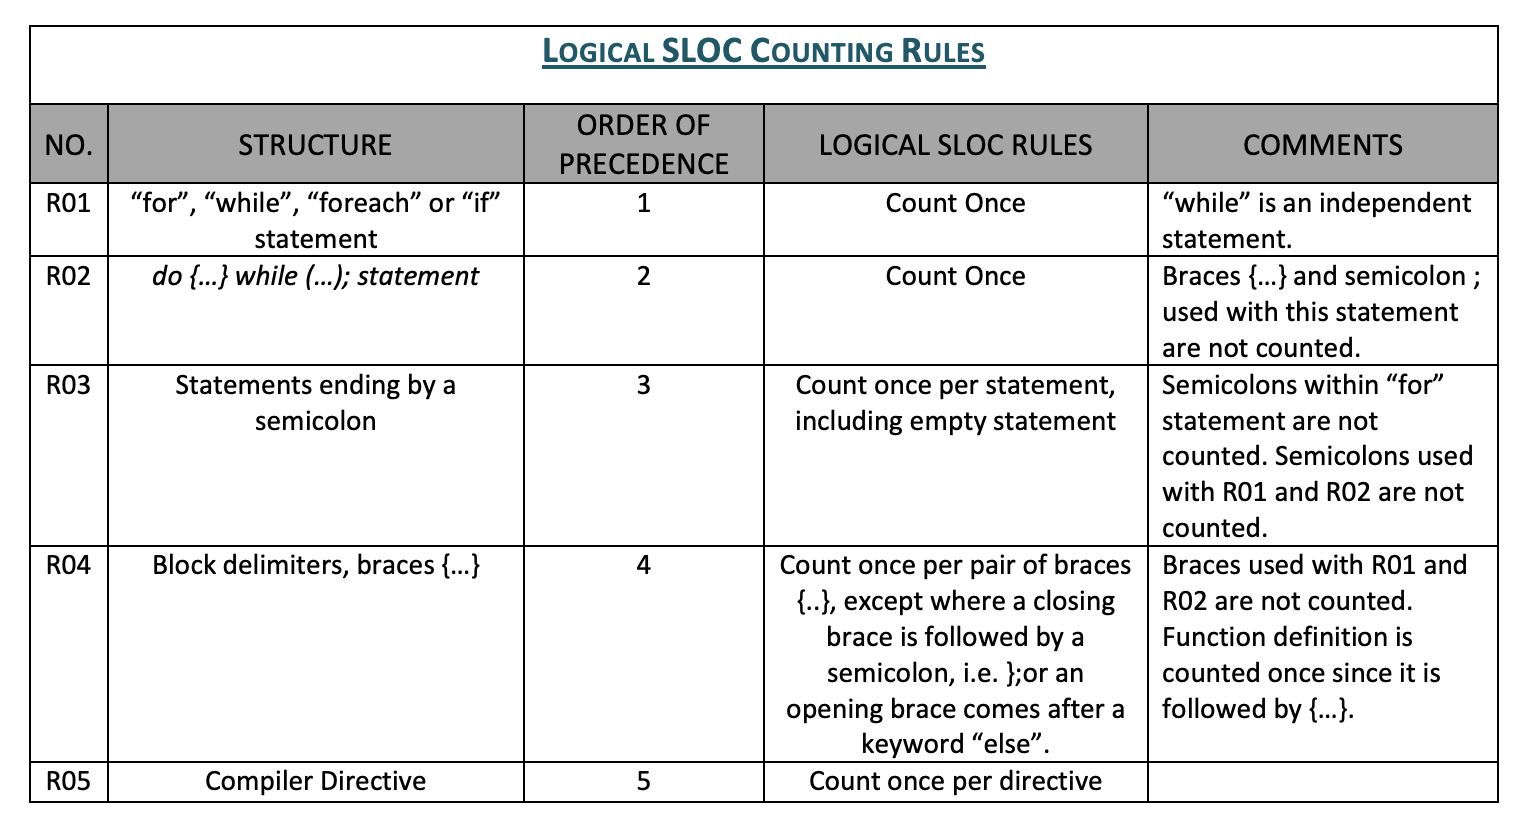
\includegraphics[width=1\linewidth]{UCC.png}
    \end{center}
       \caption{Logical SLOC Counting Rule Table\label{Logical SLOC Counting Rule Table}}
\end{figure}
\begin{figure}
    \begin{center}
    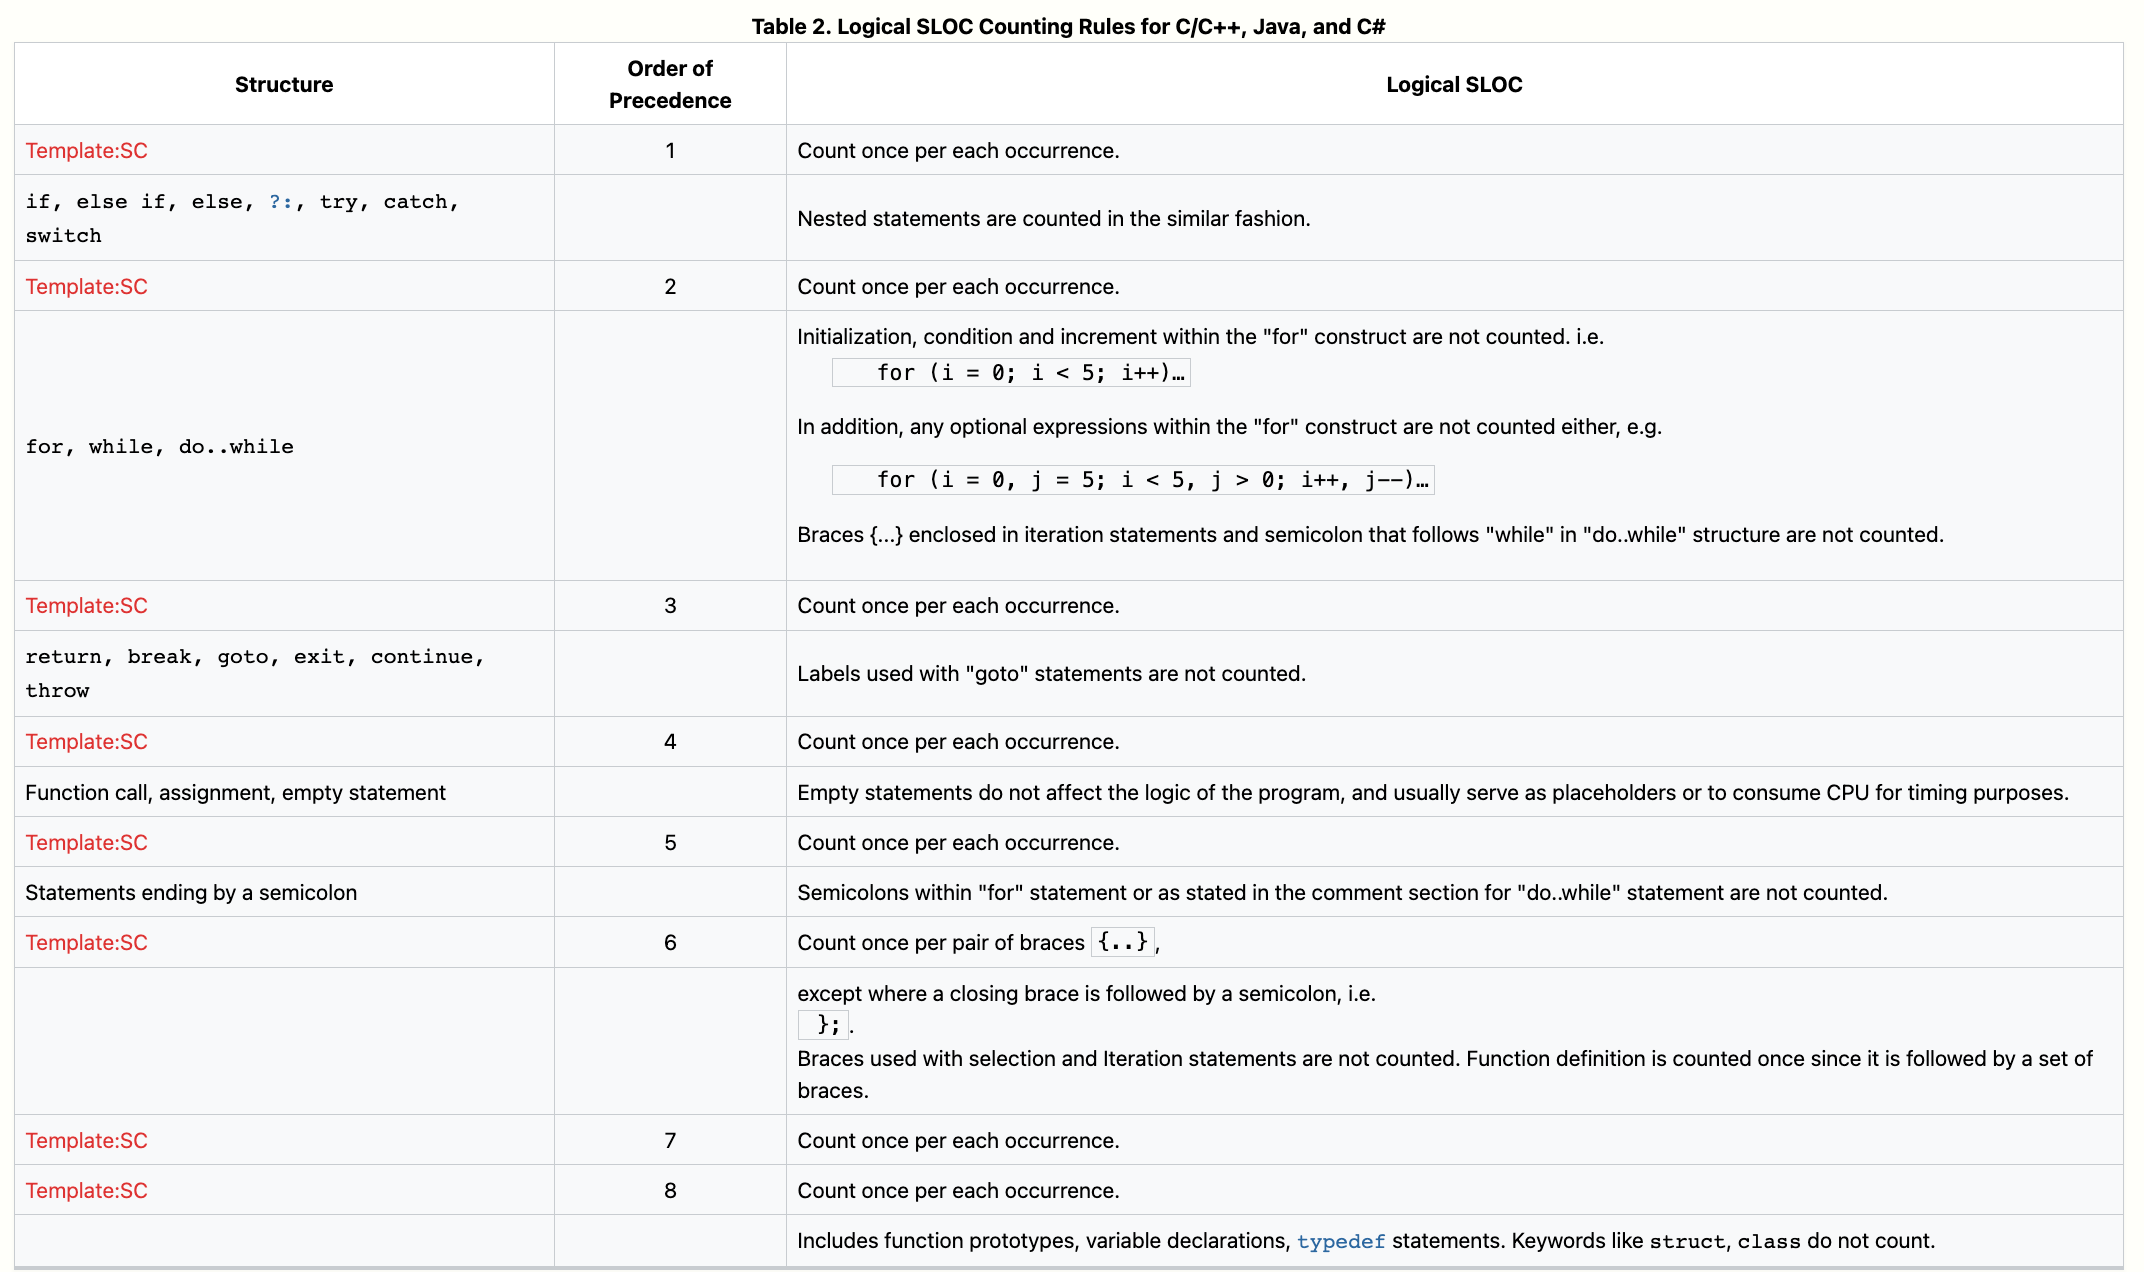
\includegraphics[width=1\linewidth]{UCC2.png}
    \end{center}
       \caption{Logical SLOC Counting Rule Table\label{Logical SLOC Counting Rule Table}}
\end{figure}
\textbf{Advantages of Logical SLOC}: Measures essential code which indicates functionality, maintainability, and performance of the code.  \\

\textbf{Inference}: In conclusion, a logical SLOC of 83 suggests that the software project is small in comparison to generic systems and may have a simpler and more manageable source code. Logical SLOC however does not provide the entire picture and so to get a more comprehensive understanding of the project, it's essential to consider other metrics and factors as well.

%%%%%%%%%%%%%%%%%%%%%%%%%%%%%%
\chapter{Problem 8 : Establishing Relation between Logical SLOC and WMC Obtained from METRICSTICS}

\section{Scatter Plot}
Figure 5.1 shows the scatter plot between the data for
Logical SLOC and WMC obtained from METRICSTICS.
By visualizing the data points on a scatter plot, we can observe patterns and trends.\\
WMC stands for "Weighted Methods per Class." It is a metric used to measure the complexity of a class and also provides an indication of how many methods within a class are present and how complex those methods are.\\
Logical SLOC is a measure of the size or complexity of a software project based on the number of logical statements or instructions in the source code that affect the program's control flow or behavior
Plotting these values on scatter plot provides us with an insight on the affect of SLOC on WMC for a given system.
\\
\begin{table}[htbp]
\centering

\begin{tabular}{|c|c|c|}
\hline
\textbf{Class} & \textbf{WMC} & \textbf{SLOC (L)} \\
\hline\hline\hline
MetricsticsApp & 0 & 9 \\
\hline
Util & 3 & 8 \\
\hline
DataGenerator & 4 & 6 \\
\hline
UIGenerator & 14 & 19 \\
\hline
Statistics & 84 & 41 \\
\hline
\end{tabular}
\caption{Class Metrics}
\end{table}
\begin{figure}
    \begin{center}
    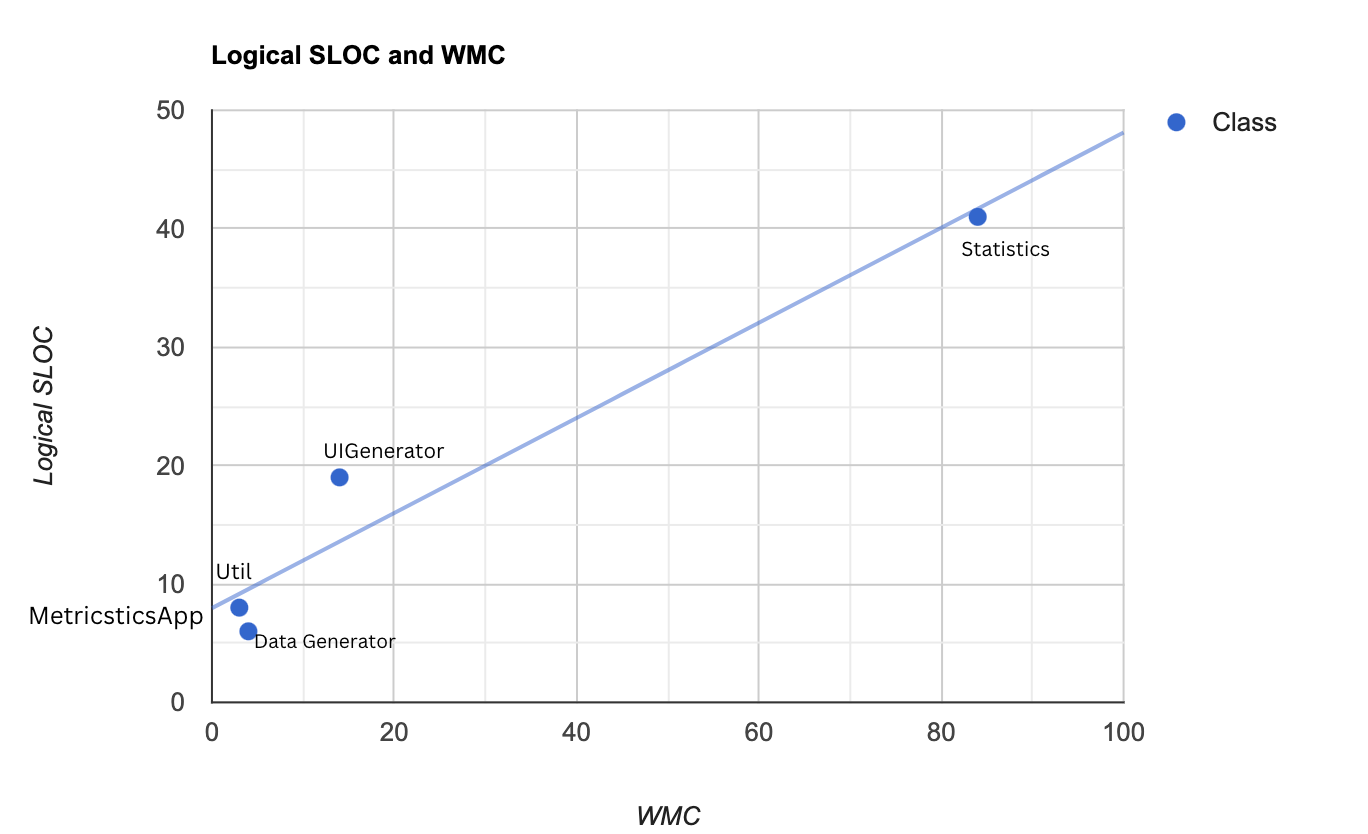
\includegraphics[width=1\linewidth]{scatterPlot.png}
    \end{center}
       \caption{Scatter Plot (Logical SLOC and WMC\label{Scatter Plot (Logical SLOC and WMC}}
\end{figure}


\\

\section{correlation coefficient}
In this section we find the correlation coefficient between WMC and SLOC(L) . By plotting the WMC values and SLOC(L) values separately on a histogram, we can conclude that these values are not normally distributed .\\
\begin{figure}
    \begin{center}
    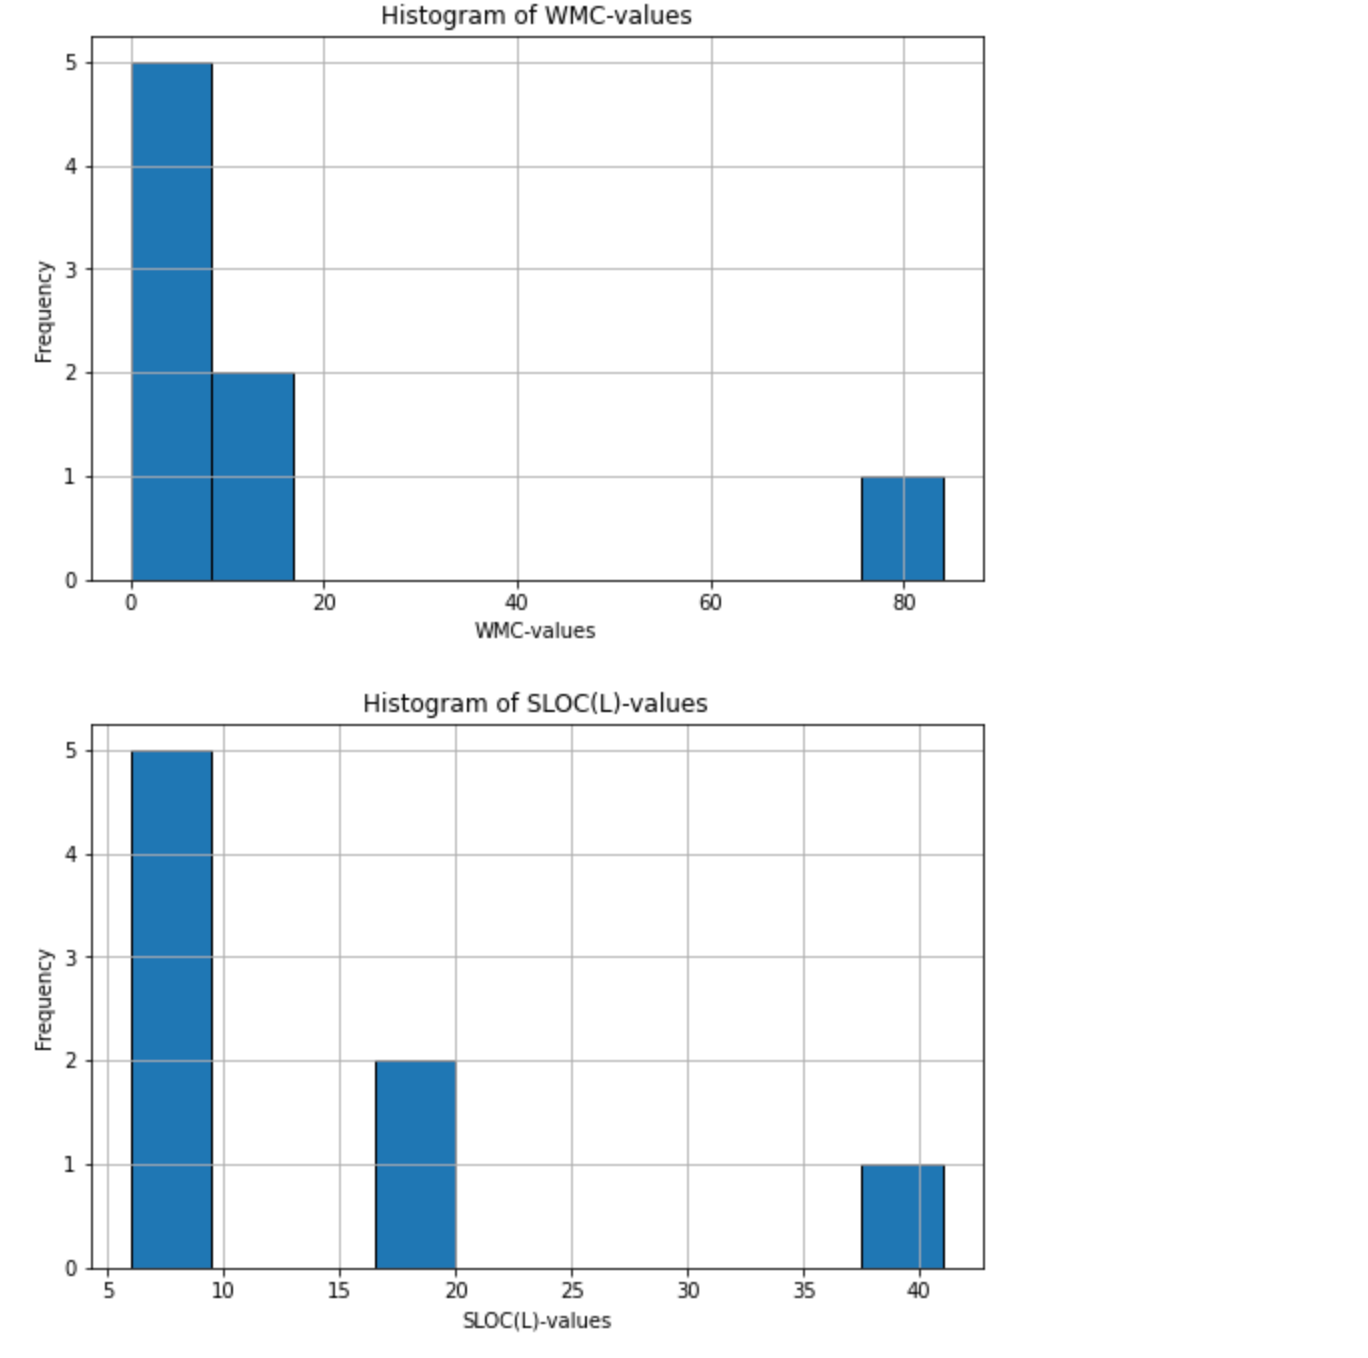
\includegraphics[width=1\linewidth]{Histo.png}
    \end{center}
       \caption{Scatter Plot (Logical SLOC and WMC\label{Scatter Plot (Logical SLOC and WMC}}
\end{figure}

Since the values of x’s [WMC] and y’s are non-normally distributed as shown in the figure[5.2], The Spearman’s Rank Correlation Coefficient (rs) can be used to find the correlation coefficient . The Spearman’s Rank Correlation Coefficient (rs) is a measure of association for attributes values that are not distributed normally [Lecture Slides]. \\
Let the data in each set of WMC(x) and SLOC(L)(y) be ranked separately in ascending order by rank (xi) and rank (yi).\\
n is the number of pairs of (x,y)\\
di = rank (xi) – rank (yi).\\
Then, rs is given by 
\[ r_{s} = 1 - \frac{6\sum_{i=n}^{n}{d^{2}_i}}{n^{3}-n} \]\\
The value of n is 5 for this particular system. All calculations are done based on the values from table 5.2\\

Spearman’s Rank Correlation Coefficient can range from -1 to 1. The closer the value is to 1 the stronger the correlation it will have. For the system of METRICSTICS the coefficient value is 0.6 which shows a strong correlation between WMC and SLOC(L).\\

The value of coefficient suggest in case the logical SLOC increases there is a high chance WMC will increase too. But conclusively we cannot say only SLOC has an impact on WMC or vice versa but many other underlying factors may also have an affect on these values. It is important to take in account all metrics of software to make justification of change.

\begin{table}[htbp]
  \centering
  
  \begin{tabular}{|c|c|c|c|c|c|}
    \hline
    $WMC(x_i)$ & Rank($x_i$) & SLOC(L)($y_i$) & Rank($y_i$) & $d$ & $d^2$ \\
    \hline\hline
    0   & 1  & 9 & 3  & -2  & 4 \\
    3  & 2  & 8 & 2  & 0  & 0 \\
    4   & 3   & 6 & 1    & 2   & 4  \\
    14   & 4   & 19 & 4  &  0  & 0 \\ 
    84   & 5   & 41 & 5   &  0  & 0 \\
    
    \hline
  \end{tabular}
  \caption{Data Table}
\end{table}



%%%%%%%%%%%%%%%%%%%%%%%%%%%%%%

\begin{thebibliography}{7}
    \addcontentsline{toc}{chapter}{Bibliography}

    % delete all of these example references, and replace them with references for your report.
    
    \bibitem{Lecture Slides} 
    Lecture Slides 
    \textit{Lecture slides"SOEN6611 Course Website”}.     
    \bibitem{Chatgpt} 
    ChatGpt
    \textit{ChatGpt}.     
    
     \bibitem{Software Measurement Metrics} 
    Metrics.,
    \\\texttt{https://www.geeksforgeeks.org/software-measurement-and-metrics/}
    
    \bibitem{Use Case Diagram} 
    Use Case Diagram.,
    \\\texttt{https://www.visual-paradigm.com/guide/uml-unified-modeling-language/what is use case diagram/}

 
      \bibitem{Physical SLOC} 
    Physical SLOC,
    \\\texttt{https://github.com/AlDanial/cloc}


      \bibitem{Logical SLOC} 
    Logical SLOC,
    \\\texttt{https://handwiki.org/wiki/Software:Unified\_Code\_Count\_(UCC)}

    \bibitem{JavaFX} 
    JavaFX,
    \\\texttt{https://en.wikipedia.org/wiki/JavaFX}



    
\end{thebibliography}

 
\textbf{{Github Repository}}

https://github.com/hemareddy123/SOEN\_6611\_Summer2023/tree/main



\end{document}